\chapter{Supplementary Material for Chapter 3: NSPPK}
\label{appendix:ch3}


\section{Computational and Space Complexity Analysis}
\label{appendix:complexity}
We analyse the computational and space complexity of NSPPK feature extraction
and kernel evaluation using the notation introduced in Chapter~\ref{ch:nsppk}.
\subsection{Notation Recap}
Let $G=(V,E)$ be a graph with $|V|=n$ nodes and $|E|=m$ edges.  
Let $K=\max_{v\in V}\deg(v)$ denote the maximum node degree and $\tau$ an optional degree cutoff.  
Let $R$ be the maximum anchor neighbourhood radius, $D$ the maximum anchor--anchor distance, and $R'$ the maximum connector radius.  
Distances are measured using unweighted shortest paths.

\subsection{Feature Extraction Time Complexity}

NSPPK feature extraction consists of two main phases.

\subsection{Neighbourhood hashing (radius $R$)}

For each node $v\in V$, we perform a breadth-first search (BFS) truncated at
depth $R$ to compute the rooted neighbourhood hash $G_H^r(v)$ for all $r\le R$.
Let
\[
\mathcal{N}_R(v)=\{u\in V : d(u,v)\le R\}
\]
denote the $R$-hop neighbourhood vertex set of $v$, and let $E_R(v)$ be the set
of edges induced by $G[\mathcal{N}_R(v)]$.

The total cost of this phase is
\[
T_{\mathrm{neigh}}
=
O\!\left(
\sum_{v\in V}\bigl(|\mathcal{N}_R(v)| + |E_R(v)|\bigr)
\right).
\]

In the worst case (e.g., when $R$ exceeds the graph diameter),
\[
T_{\mathrm{neigh}} = O\bigl(n(n+m)\bigr).
\]

For fixed $R$ on bounded-degree graphs, $|\mathcal{N}_R(v)| = O(K^R)$, yielding
\[
T_{\mathrm{neigh}} = O\bigl(n K^{R+1}\bigr),
\]
or $O\bigl(n K_{\mathrm{eff}}^{R+1}\bigr)$ when a degree cutoff
$K_{\mathrm{eff}}=\min(K,\tau)$ is applied.

Each neighbourhood hash is computed once per node and reused during pairwise feature construction.

\subsection{Pairwise enumeration up to distance $D$}

For each node $v\in V$, we run a BFS truncated at depth $D$ to enumerate all nodes $u$ such that $d(v,u)\le D$.  
For each such pair $(v,u)$, we generate pairwise features combining:
(i) the precomputed neighbourhood hashes $G^r_H(v)$ and $G^r_H(u)$,
(ii) the distance $d(v,u)$,
and (iii) optionally the connector
$C_{r'}(v,u)=G[\mathcal{N}_{r'}(V(U(v,u)))]$.

Once the constituent neighbourhood and connector encodings have been computed,
combining their fixed-width hash values requires constant time for a fixed
feature-tuple length. This does not include the cost of constructing the
connector encoding itself.
The total cost of this phase is
\[
T_{\mathrm{pairs}}
=
O\!\left(
\sum_{v\in V}\bigl(|\mathcal{N}_D(v)| + |E_D(v)|\bigr)
\right).
\]

Worst-case complexity is
\[
T_{\mathrm{pairs}} = O\bigl(n(n+m)\bigr),
\]
with $\Theta(n^2)$ pairwise features generated in dense or small-diameter graphs.

For fixed $D$ and bounded degree,
\[
T_{\mathrm{pairs}} = O\bigl(n K^{D+1}\bigr),
\]
or $O\bigl(n K_{\mathrm{eff}}^{D+1}\bigr)$ with degree cutoff.


\subsection{Total feature extraction cost}

Combining neighbourhood hashing, anchor-pair enumeration, and connector
construction gives
\[
T_{\mathrm{total}}
=
O\!\left(
\sum_{v\in V}
\bigl(|\mathcal{N}_R(v)|+|E_R(v)|\bigr)
+
\sum_{v\in V}
\bigl(|\mathcal{N}_D(v)|+|E_D(v)|\bigr)
+
C_{\mathrm{conn}}
\right),
\]
where $C_{\mathrm{conn}}$ denotes the total cost of constructing and encoding
the connector structures associated with the enumerated anchor pairs.

For fixed parameters $(R,D,R')$, bounded effective degree, and connector
construction restricted to bounded local regions, the total cost is
near-linear in $|V|$. In dense or small-diameter graphs, however, the number
and size of the relevant anchor configurations may approach a quadratic
regime. The worst-case cost therefore remains
\[
O\!\bigl(n(n+m)+C_{\mathrm{conn}}\bigr).
\]

\subsection{Attribute Integration Cost}

Let each node carry a $p$-dimensional attribute vector. Structural feature
extraction is independent of $p$. Once a structural feature occurrence has
been identified, aggregating the attributes of its participating nodes incurs
a cost linear in $p$.

If $N_{\mathrm{inc}}$ denotes the total number of node--feature incidences
processed during attribute aggregation, then
\[
T_{\mathrm{attr}}=O(pN_{\mathrm{inc}}),
\]
and the overall cost is
\[
T_{\mathrm{total}}
=
T_{\mathrm{struct}}+O(pN_{\mathrm{inc}}).
\]
Thus, attribute integration scales linearly with the attribute dimension but
does not multiply the cost of the graph searches themselves.

\subsection{Kernel Evaluation Complexity}

Once feature extraction is complete, each graph $G$ is represented by a sparse feature-count vector $f_G^\theta$.  
Kernel evaluation reduces to a sparse dot product
\[
k_\theta(G,G') = {f_G^\theta}^{\top}f_{G'}^\theta,
\]
with time complexity
\[
O\bigl(\mathrm{nnz}(f_G^\theta) + \mathrm{nnz}(f_{G'}^\theta)\bigr),
\]
where $\mathrm{nnz}(\cdot)$ denotes the number of non-zero entries.  
In practice, kernel evaluation scales near-linearly with
$\mathrm{nnz}(f_G^\theta)$ for fixed radii and bounded degree, while dense or high-degree graphs may induce quadratic feature growth.


\subsection{Space Complexity}

The space requirements of NSPPK are as follows:
\begin{itemize}
\item Neighborhood hashes: $O(n)$.
\item BFS working memory: $O(n)$ in the worst case (reused across runs).
\item Feature vectors: $O(F)$, where $F$ is the number of distinct hashed features observed.  
In the worst case, $F=O(n^2)$, but in practice sparsity is maintained due to small $R,D$, degree cutoffs, and hashing.
\item Attribute-augmented features: $O(pF)$ in a dense representation, but stored sparsely as accumulated sums.
\end{itemize}

\subsection{Summary}

Under typical settings with small radii and bounded effective degree, NSPPK achieves near-linear feature extraction time in $|V|$, linear kernel evaluation time in the number of active features, and explicit sparse representations with predictable memory usage.  
The worst-case bounds coincide with those of other pairwise-distance-based kernels and reflect the intrinsic cost of enumerating all relevant node pairs.


\section{Datasets}
\label{appendix:datasets}

The graphs are undirected, with nodes labelled, attributed, or both. All datasets are publicly accessible \cite{kersting2016benchmark,morris2020tudataset} and have been widely used in comparative studies of graph kernels and GNNs \cite{nikolentzos2021graph}.

\textbf{BZR} consists of 405 chemical compounds represented as graphs, where nodes correspond to atoms and edges to chemical bonds. The task is to predict whether a compound acts as a ligand for the benzodiazepine receptor \cite{Dobson2003DistinguishingES}.

\textbf{COX2} contains 467 molecules represented as graphs, labelled according to their activity against the cyclooxygenase-2 enzyme (COX-2 inhibitor classification) \cite{Dobson2003DistinguishingES}.

\textbf{ENZYMES} consists of 600 protein tertiary structures from the BRENDA database. Each protein belongs to one of six top-level enzyme commission (EC) classes, and the task is to predict the correct class \cite{borgwardt2005protein}.

\textbf{PROTEINS} and \textbf{PROTEINS\_full} represent proteins as graphs, where vertices correspond to secondary structure elements. Edges connect vertices that are adjacent in the amino acid sequence or in 3D space. The classification task is to distinguish enzymes from non-enzymes \cite{borgwardt2005protein}.

\textbf{SYNTHETICnew} contains 300 synthetic graphs evenly split into two classes. Each graph has 100 vertices and 196 edges with normally distributed node attributes. Class 1 graphs are generated by rewiring 5 edges and permuting 10 node attributes; Class 2 graphs by rewiring 10 edges and permuting 5 attributes. Gaussian noise is added to all attributes \cite{shervashidze2011weisfeiler}.



\textbf{DHFR}
contains 756 molecules represented as graphs, labelled according to their activity against the dihydrofolate reductase (DHFR) enzyme \cite{sutherland2003spline}

\begin{table}[h]
\centering
\caption{Dataset statistics.}
\label{tab:dataset_stats}
\scriptsize
\setlength{\tabcolsep}{4.2pt}
\begin{adjustbox}{max width=\linewidth}
\begin{tabular}{lccccccc}
\toprule
\textbf{Dataset} & \#Graphs & \#Classes / Tasks & Avg.\ |V| & Avg.\ |E| & Avg.\ deg. & Max deg. & Attr.\ dim. \\
\midrule
BZR            & 405     & 2   & 35.75 & 38.36 & 2.15 & 4  & 3  \\
COX2           & 467     & 2   & 41.23 & 43.45 & 2.11 & 4  & 3  \\
ENZYMES        & 600     & 6   & 32.63 & 62.14 & 3.86 & 9  & 18 \\
PROTEINS\_full & 1113    & 2   & 39.06 & 72.82 & 3.74 & 25 & 1  \\
SYNTHETICnew   & 300     & 2   & 100.00& 196.25& 3.93 & 9  & 1  \\
DHFR           & 756     & 2   & 42.43 & 44.54 & 2.10 & 5  & 3  \\
ogbg-molpcba   & 437{,}929 & 128 & 25.96 & 28.10 & 2.16 & 4  & 9  \\
\bottomrule
\end{tabular}
\end{adjustbox}
\end{table}


\section{Hyperparameters used for model selection in the graph classification task}
\label{appendix:hyperparameters}

For some kernels, only a subset of the hyperparameters
was optimised, while the rest of the hyperparameters were kept fixed.

\begin{table}[H]
    \centering
    \caption{Hyperparameters used for model selection in the graph classification experiments .}
    \scriptsize
    \renewcommand{\arraystretch}{1.2}
    \setlength{\tabcolsep}{3pt}
    \begin{adjustbox}{max width=\textwidth}
    \begin{tabular}{lcccccccccccccc}
        \toprule
        \textbf{Model} &
        \textbf{Layers} &
        \makecell{\textbf{Convs}\\\textbf{per layer}} &
        \makecell{\textbf{Batch}\\\textbf{size}} &
        \makecell{\textbf{Learning}\\\textbf{rate}} &
        \makecell{\textbf{Hidden}\\\textbf{units}} &
        \textbf{Epochs} &
        \textbf{L2} &
        \textbf{Dropout} &
        \makecell{\textbf{Patience}\\\textbf{(loss, acc)}} &
        \textbf{Optimizer} &
        \textbf{Scheduler} &
        \makecell{\textbf{Dense}\\\textbf{dim}} &
        \makecell{\textbf{Embed.}\\\textbf{dim}} &
        \makecell{\textbf{Neighbours}\\\textbf{Aggregation}} \\
        \midrule
        DGNN & 2,3,4 & 1 & 16 & $1\mathrm{e}{-4}$ & 32, 64 & 1000 & -- & 0.5 &
        \makecell{500, 500} & Adam & -- & 128 & -- & mean, max, sum \\
        GIN & \makecell{see\\hidden units} & 1 & 32, 128 & $1\mathrm{e}{-2}$ &
        \makecell{32 (5 layers),\\64 (5 layers),\\64 (2 layers),\\32 (3 layers)} &
        1000 & -- & 0, 0.5 & \makecell{500, 500} &
        Adam & \makecell{StepLR\\(step 50, $\gamma{=}0.5$)} & -- & -- & sum \\
        GraphSAGE & 3, 5 & 1 & 16 & $1\mathrm{e}{-2},\,1\mathrm{e}{-3},\,1\mathrm{e}{-4}$ &
        32, 64 & 1000 & -- & 0 & \makecell{500, 500} & Adam & -- & -- & -- &
        mean, max, sum \\
        InfoGraph & 3, 5 & -- & 16, 32 & $1\mathrm{e}{-2},\,1\mathrm{e}{-3}$ &
        32, 64, 128 & 100 & \makecell{0, $1\mathrm{e}{-4}$} & 0, 0.1, 0.3 &
        \makecell{500, 500} & Adam & \makecell{ReduceLROnPlateau\\($\gamma{=}0.5$)} &
        -- & -- & sum \\
        GNN & 3, 5 & 1 & 16 & $1\mathrm{e}{-2},\,1\mathrm{e}{-3},\,1\mathrm{e}{-4}$ &
        32, 64 & 1000 & -- & 0, 0.5 & \makecell{500, 500} &
        Adam & \makecell{StepLR\\(step 50, $\gamma{=}0.5$)} & -- & -- &
        mean, max, sum \\
        GraphCL & 2, 3 & 1 & 32 & $1\mathrm{e}{+3}$ & 64, 128 & 200 & -- & 0 &
        \makecell{500, 500} & Adam & -- & -- & -- & mean, max, sum \\
        FNP & 2, 3, 4 & 1 & 32 & $1\mathrm{e}{-3}$ & 32, 64 & 1000 & -- &
        0.0, 0.2, 0.5 & \makecell{500, 500} & Adam & -- & -- & -- & sum \\
        PNA & 2, 3, 2 & 1 & 32 & $1\mathrm{e}{-3}$ & 32, 64 & 1000 & -- & 0 &
        \makecell{500, 500} & Adam & -- & -- & -- & max \\
        PDF & 2, 3 & 1 & 32 & $5\mathrm{e}{-4}$ & 64, 129 & 300 & $1\mathrm{e}{-2}$ &
        0 & \makecell{500, 500} & Adam & \makecell{StepLR\\(step 50, $\gamma{=}0.5$)} &
        -- & -- & mean \\
        \bottomrule
    \end{tabular}
    \end{adjustbox}
\end{table}
\begin{table}[H]
    \centering
    \footnotesize  % <-- smaller than \small
    \renewcommand{\arraystretch}{1.2}
    \caption{Hyperparameters used in the kernels for model selection in the graph classification task.}
    \label{tab:hyperparameters}
    \begin{tabular}{l p{3.5cm} p{8.5cm}}
        \toprule
        \textbf{Kernel} & \textbf{Fixed} & \textbf{Validation-tuned} \\
        \midrule
        SM & $k = 3$ & -- \\
        SP & -- & -- \\
        ML & $\gamma = 0.01$, $\eta = 0.01$, $\hat{p} = 10$ & $l_{\max} \in \{0,\dots,5\}$, $\tilde{c} \in \{50,100,200,300\}$ \\
        PK & $w = 10^{-5}$ & $T \in \{1,\dots,6\}$ \\
        HSPPK-WL & Iterations = 20  & $h \in \{0,\dots,5\}$ \\
        HSPPK-SP & Iterations = 20  & $h \in \{0,\dots,5\}$ \\
        GH & -- & Linear kernel / Gaussian kernel \\
        linearFGW-RAW & RBF kernel, $\gamma = 0.1$ & $\alpha \in \{0.1, 0.5, 0.9\}$, GWB layers $= 5$, OT layers $\in \{3,5\}$, Iter $\in \{1,2,3\}$, $\gamma_{\text{kernel}} \in \{0.01, 0.1, 1.0\}$ \\
        linearFGW-WL1 & RBF kernel, $\gamma = 0.1$ & same as above \\
        linearFGW-WL2 & RBF kernel, $\gamma = 0.1$ & same as above \\
        WL (disc) & -- & Iterations $\in \{0,\dots,5\}$ \\
        WLOA & -- & Iterations $\in \{0,\dots,5\}$ \\
        WWL & -- & Iterations $\in \{0,\dots,7\}$, Sinkhorn $\in \{\texttt{False}, \texttt{True}\}$, $\gamma \in \{0.01, 0.1, 1, 10\}$ \\
        NP & -- & Iterations $\in \{0,\dots,5\}$, Linear / Gaussian kernel \\
        NSPDK & $D = 1$, $R = 4$ & -- \\
        NSPDK (disc) & $D = 1$, $R = 4$ & -- \\
        NSPPK & \multicolumn{2}{p{12cm}}{\centering $D = 1$, $R = 4$, $R' = 1$,threshold $\tau = 8$, hash bits $b = 16$} \\
        \bottomrule
    \end{tabular}
\end{table}


\section{Robustness Study Hyperparameters}
\label{appendix:robustness}

Table~\ref{tab:robustness-hparams} summarizes the configurations used for the
diagonal-dominance and robustness experiments in
Section~\ref{sec:Diagonal}.
Neural baselines (GIN-Random, GraphCL, InfoGraph) were run with a common lightweight setup , while classical kernels (GraphHopper, Propagation Kernel) followed their standard definitions. NSPPK used the same fixed configuration as in the main experiments.

\begin{table}[H]
\centering
\caption{Hyperparameters for robustness / diagonal dominance analysis.}
\label{tab:robustness-hparams}
\renewcommand{\arraystretch}{1.1}
\setlength{\tabcolsep}{6pt}
\begin{tabular}{p{3.2cm} p{9.5cm}}
\toprule
\textbf{Method} & \textbf{Configuration} \\
\midrule
\textbf{NSPPK} & $R=1$, $D=4$, $R'=1$, $\tau=8$, $b=12$ \\
\textbf{GIN-Random} & 3 layers GIN, hidden dim=32, MLP layers=2, pooling=sum, epochs=200, lr=0.01, seed=42, orthogonal init, no supervision \\
\textbf{GraphCL} & Same GIN backbone as above, contrastive pretraining with augmentations, 200 epochs, lr=0.01 \\
\textbf{InfoGraph} & Same GIN backbone as above, maximizing mutual information, 200 epochs, lr=0.01 \\
\textbf{GraphHopper} & Shortest-path kernel, weight decay $w=10^{-5}$, $t_{\max} \in \{1,2,3,4,5\}$ \\
\textbf{Propagation Kernel} & Attribute propagation with $M=L1$ distance, 5 iterations \\
\bottomrule
\end{tabular}
\end{table}



For InfoGraph, GraphCL, and GIN-Random, we generate a synthetic dataset of
50{,}000 graphs similar to the prototype graph $G$, with the number of nodes
ranging from 50 to 250, allowing the models to detect node-dropping
perturbations.

\section{Large scale embedding experiment: QM9}
\label{appendix:qm9}

\begin{figure}[H]
    \centering
    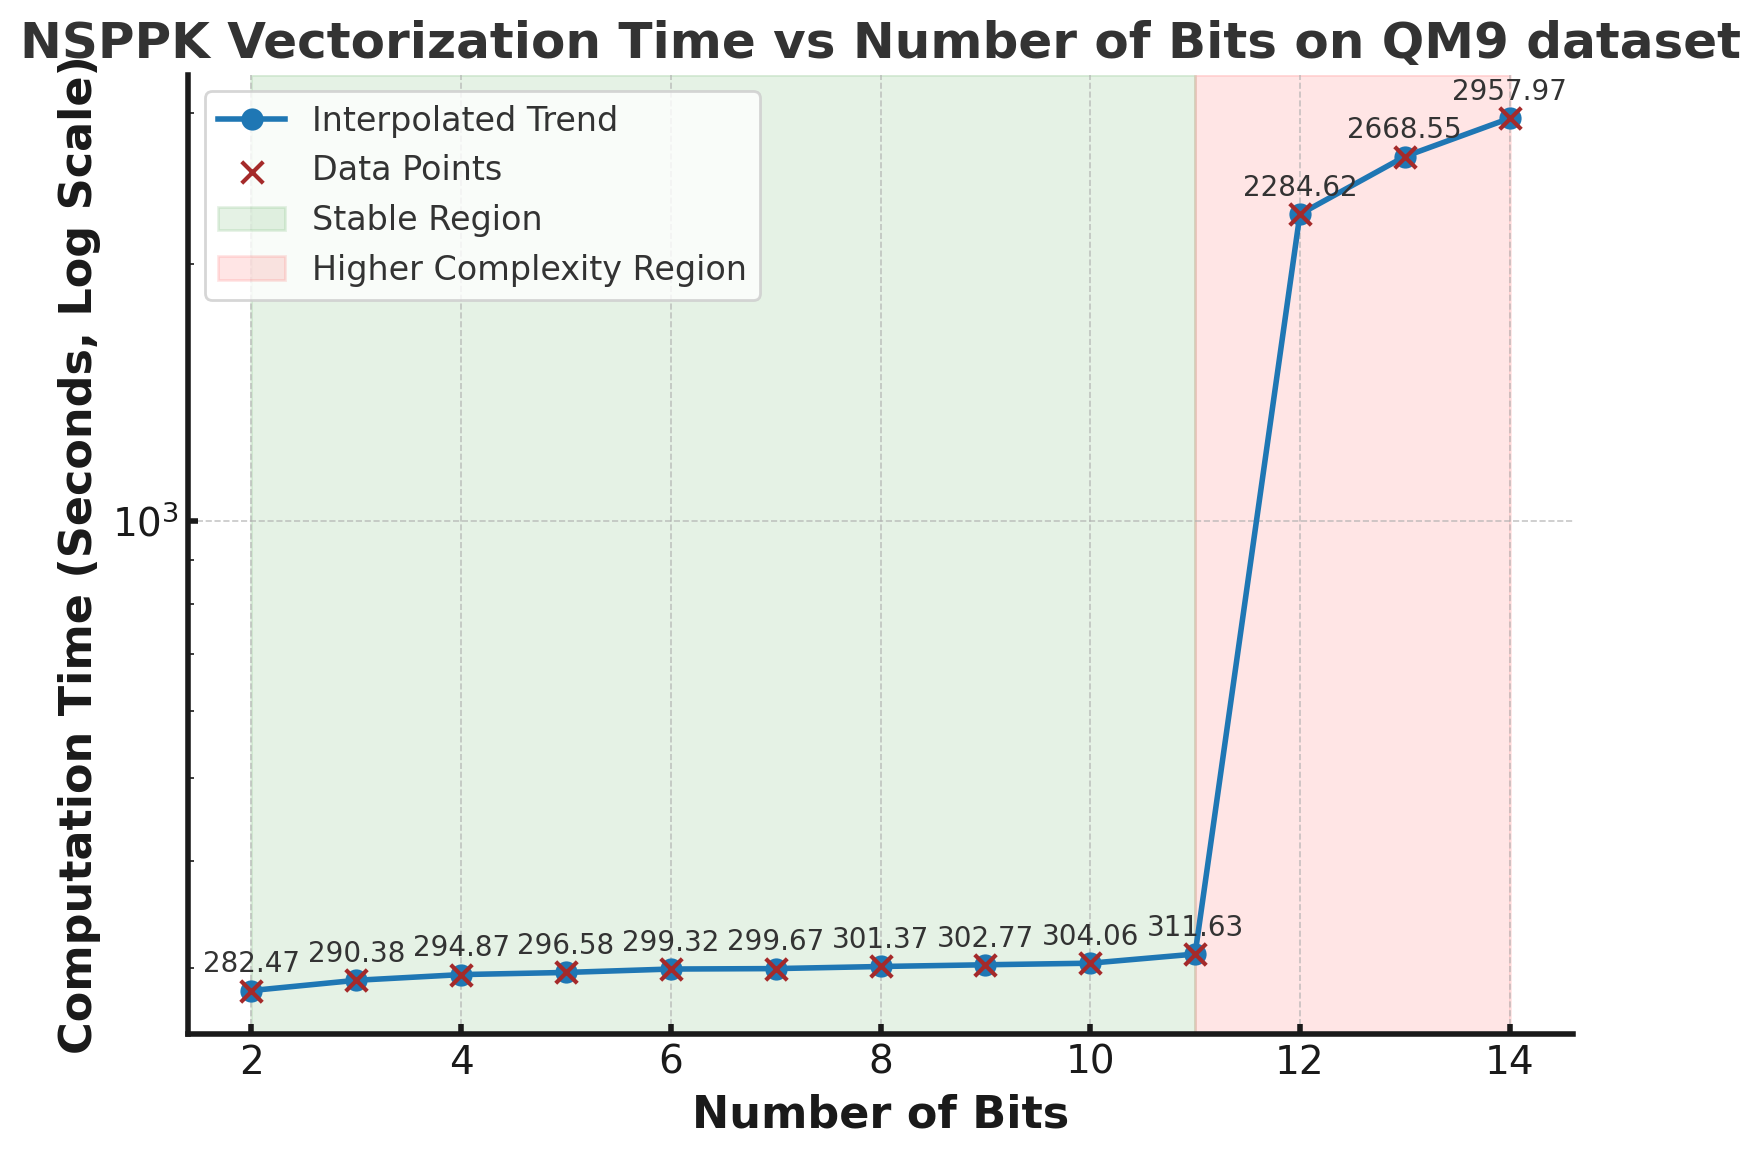
\includegraphics[width=0.8\textwidth]{images/qm9_plot.png}
    \caption{NSPPK vectorisation time for QM9 dataset as a function of number of bits.}
    \label{fig:nsppk_qm9}
\end{figure}

Figure \ref{fig:nsppk_qm9} illustrates the time required for NSPPK to vectorize the QM9 \cite{blum2009gdb13} dataset as a function of the number of hash bits $b$. As the number of bits increases, the vectorisation time rises accordingly, though the rate of increase is not uniform. Up to 11 bits, the computation time remains within a small range (under 7 minutes), demonstrating NSPPK’s efficiency in handling large-scale datasets.

However, a sharp increase in computation time occurs from 12 to 14 bits due to memory swapping, where the system resorts to using slower secondary storage instead of RAM. This significantly degrades performance, further emphasising the importance of efficient memory usage when handling high-bit representations in large-scale datasets.

At $b=15$, the vectorisation process fails due to excessive memory allocation requirements. This is a consequence of the exponential growth of the feature space: $b=15$ corresponds to a \(2^{15}\)-dimensional hash codomain, resulting in an immense memory footprint when applied to over 129,000 molecular graphs. While this represents a practical upper bound for single-machine processing, it highlights the need for optimised memory management strategies for ultra-high-dimensional embeddings.

Despite this limitation, NSPPK remains an effective and scalable approach for graph learning tasks, provided that memory usage is carefully managed when selecting the number of bits. Additionally, potential optimisations such as sparse representations, dimensionality reduction, or distributed processing could further enhance its applicability to even larger datasets.

The QM9 dataset itself consists of over 129,000 molecular graphs with 16 continuous node attributes, making it a computationally intensive benchmark. The results confirm that NSPPK successfully processes datasets of this magnitude while maintaining practical computation times, reinforcing its utility for real-world graph-based applications.


\section{Additional Experiments on Citation Networks}
\label{appendix:citation}

To further evaluate the robustness of NSPPK beyond molecular graphs,
we conducted experiments on three widely used citation network
benchmarks: \textbf{Cora}, \textbf{CiteSeer}, and \textbf{PubMed}.
These graphs exhibit higher-degree outliers, broader graph diameters,
and citation-style connectivity patterns, in contrast to the smaller
and sparser molecular graphs considered elsewhere in this work.

\begin{table}[h]
\centering
\caption{Citation network statistics and NSPPK encoding time.}
\scriptsize
\setlength{\tabcolsep}{4pt}
\begin{tabular}{lrrrrr}
\toprule
Dataset & \#Nodes & \#Edges & Avg Deg. & Max Deg. & Encoding Time (s) \\
\midrule
Cora     & 2{,}708  & 5{,}278  & 3.90 & 168 & 0.7897 \\
Citeseer & 3{,}327  & 4{,}552  & 2.74 & 99  & 0.7447 \\
PubMed   & 19{,}717 & 44{,}324 & 4.50 & 171 & 0.8747 \\
\bottomrule
\end{tabular}
\end{table}

\paragraph{Baselines.}
We compared NSPPK against a set of commonly used graph neural
network architectures for node classification:
GCN~\citep{kipf2017semi},
GAT~\citep{velivckovic2018gat},
GraphSAGE~\citep{hamilton2017graphsage},
GIN~\citep{xu2019powerful},
SGC~\citep{wu2019simplifying},
APPNP~\citep{klicpera2019predict},
and a feature-only MLP baseline.

\paragraph{Neural model configuration.}
All GNN models were trained on the original citation graphs using
the same 80/20 train--test split as NSPPK.

For GCN, GIN, GraphSAGE, and GAT we used two-layer architectures
with hidden dimension 64, ReLU activations, and dropout between
layers. GAT employed eight attention heads in the first layer.

APPNP was implemented as a two-layer MLP followed by personalized
PageRank propagation with $K=10$ steps and teleport probability
$\alpha=0.1$. SGC used a single linear classifier with $K=2$
propagation steps.

All models were trained using the Adam optimizer
(learning rate 0.01, weight decay $5\times10^{-4}$) for 200 epochs.
Model selection relied solely on the fixed training split,
without dataset-specific hyperparameter tuning.
Performance is reported using macro-averaged ROC--AUC.

\paragraph{NSPPK configuration.}
For the citation-network experiments, we retained the same general NSPPK
construction but used $R=1$, $D=4$, $R'=0$, and 11-bit hashing.

Continuous node attributes were projected to 24 dimensions using SVD.
Because NSPPK requires discrete node labels, we applied $k$-means
clustering with $k=5$ on the node attribute vectors and assigned
cluster memberships as node labels.


\section{Large-Scale Experiment: MolPCBA Learning Curves and Efficiency}
\label{appendix:molpcba}

We evaluated NSPPK on the large-scale \texttt{ogbg-molpcba} benchmark from the Open Graph Benchmark suite \cite{hu2020ogb}, which includes  437,929 node attributed molecular graphs and 128 binary classification tasks.  
In practice, many of these tasks are both sparse (due to missing labels) and highly imbalanced.





\section{Case Study: Target 95 from \texttt{ogbg-molpcba}}
We further examined \textbf{task~95}, which provides 48,853 positive examples, 293,968 negatives, and 95,108 molecules with missing labels. 
To analyze sample efficiency, we subsampled balanced datasets up to \textbf{78,164 labelled graphs} (positives and negatives in equal proportion) and varied the training set size from 100 to 250k examples.  
Each experiment was repeated with \textbf{five random seeds}, and average precision (AP) was reported.  
In parallel, we also trained each baseline once on the \emph{full OGB scaffold split} (249,715 train, 29,826 validation, 29,427 test).  

We compared NSPPK in combination with different downstream classifiers—logistic regression, random forest, and XGBoost—using both \emph{sparse} and \emph{dense} feature representations, against neural baselines including GIN, GAT, PNA, PDF, a generic GNN, and AttentiveFP (FNP).  
The distinction between sparse and dense refers only to feature storage: sparse matrices retain only nonzeros and are CPU-efficient, while dense mode expands full vectors (more memory, but occasionally favourable for GPU kernels).

For NSPPK, we fixed a single configuration (\(R=1\), \(D=4\), \(R'=1\), \(n_{\text{bits}}=16\)) across all runs.  (see Appendix~\ref{appendix:task95} for full implementation details of the graph neural networks models used within this experiment).


Figure~\ref{fig:appendix_large_experiment} summarizes the results.  
NSPPK shows strong sample efficiency, achieving higher AP than all neural baselines at small training sizes.  
Its runtime is also favourable: sparse variants in particular remain substantially faster to train than graph neural networks.  
At scale, PDF overtakes NSPPK in predictive performance, though the gap remains small.  
Interestingly, NSPPK combined with logistic regression can take as long as a GNN to train, but still delivers superior AP on small data regimes.  
Overall, NSPPK offers a simple, lightweight alternative that competes directly with neural methods.
Figure~\ref{fig:appendix_large_experiment} shows the resulting learning curves, with all NSPPK variants highlighted in red.  
\begin{figure}[H]
  \centering
  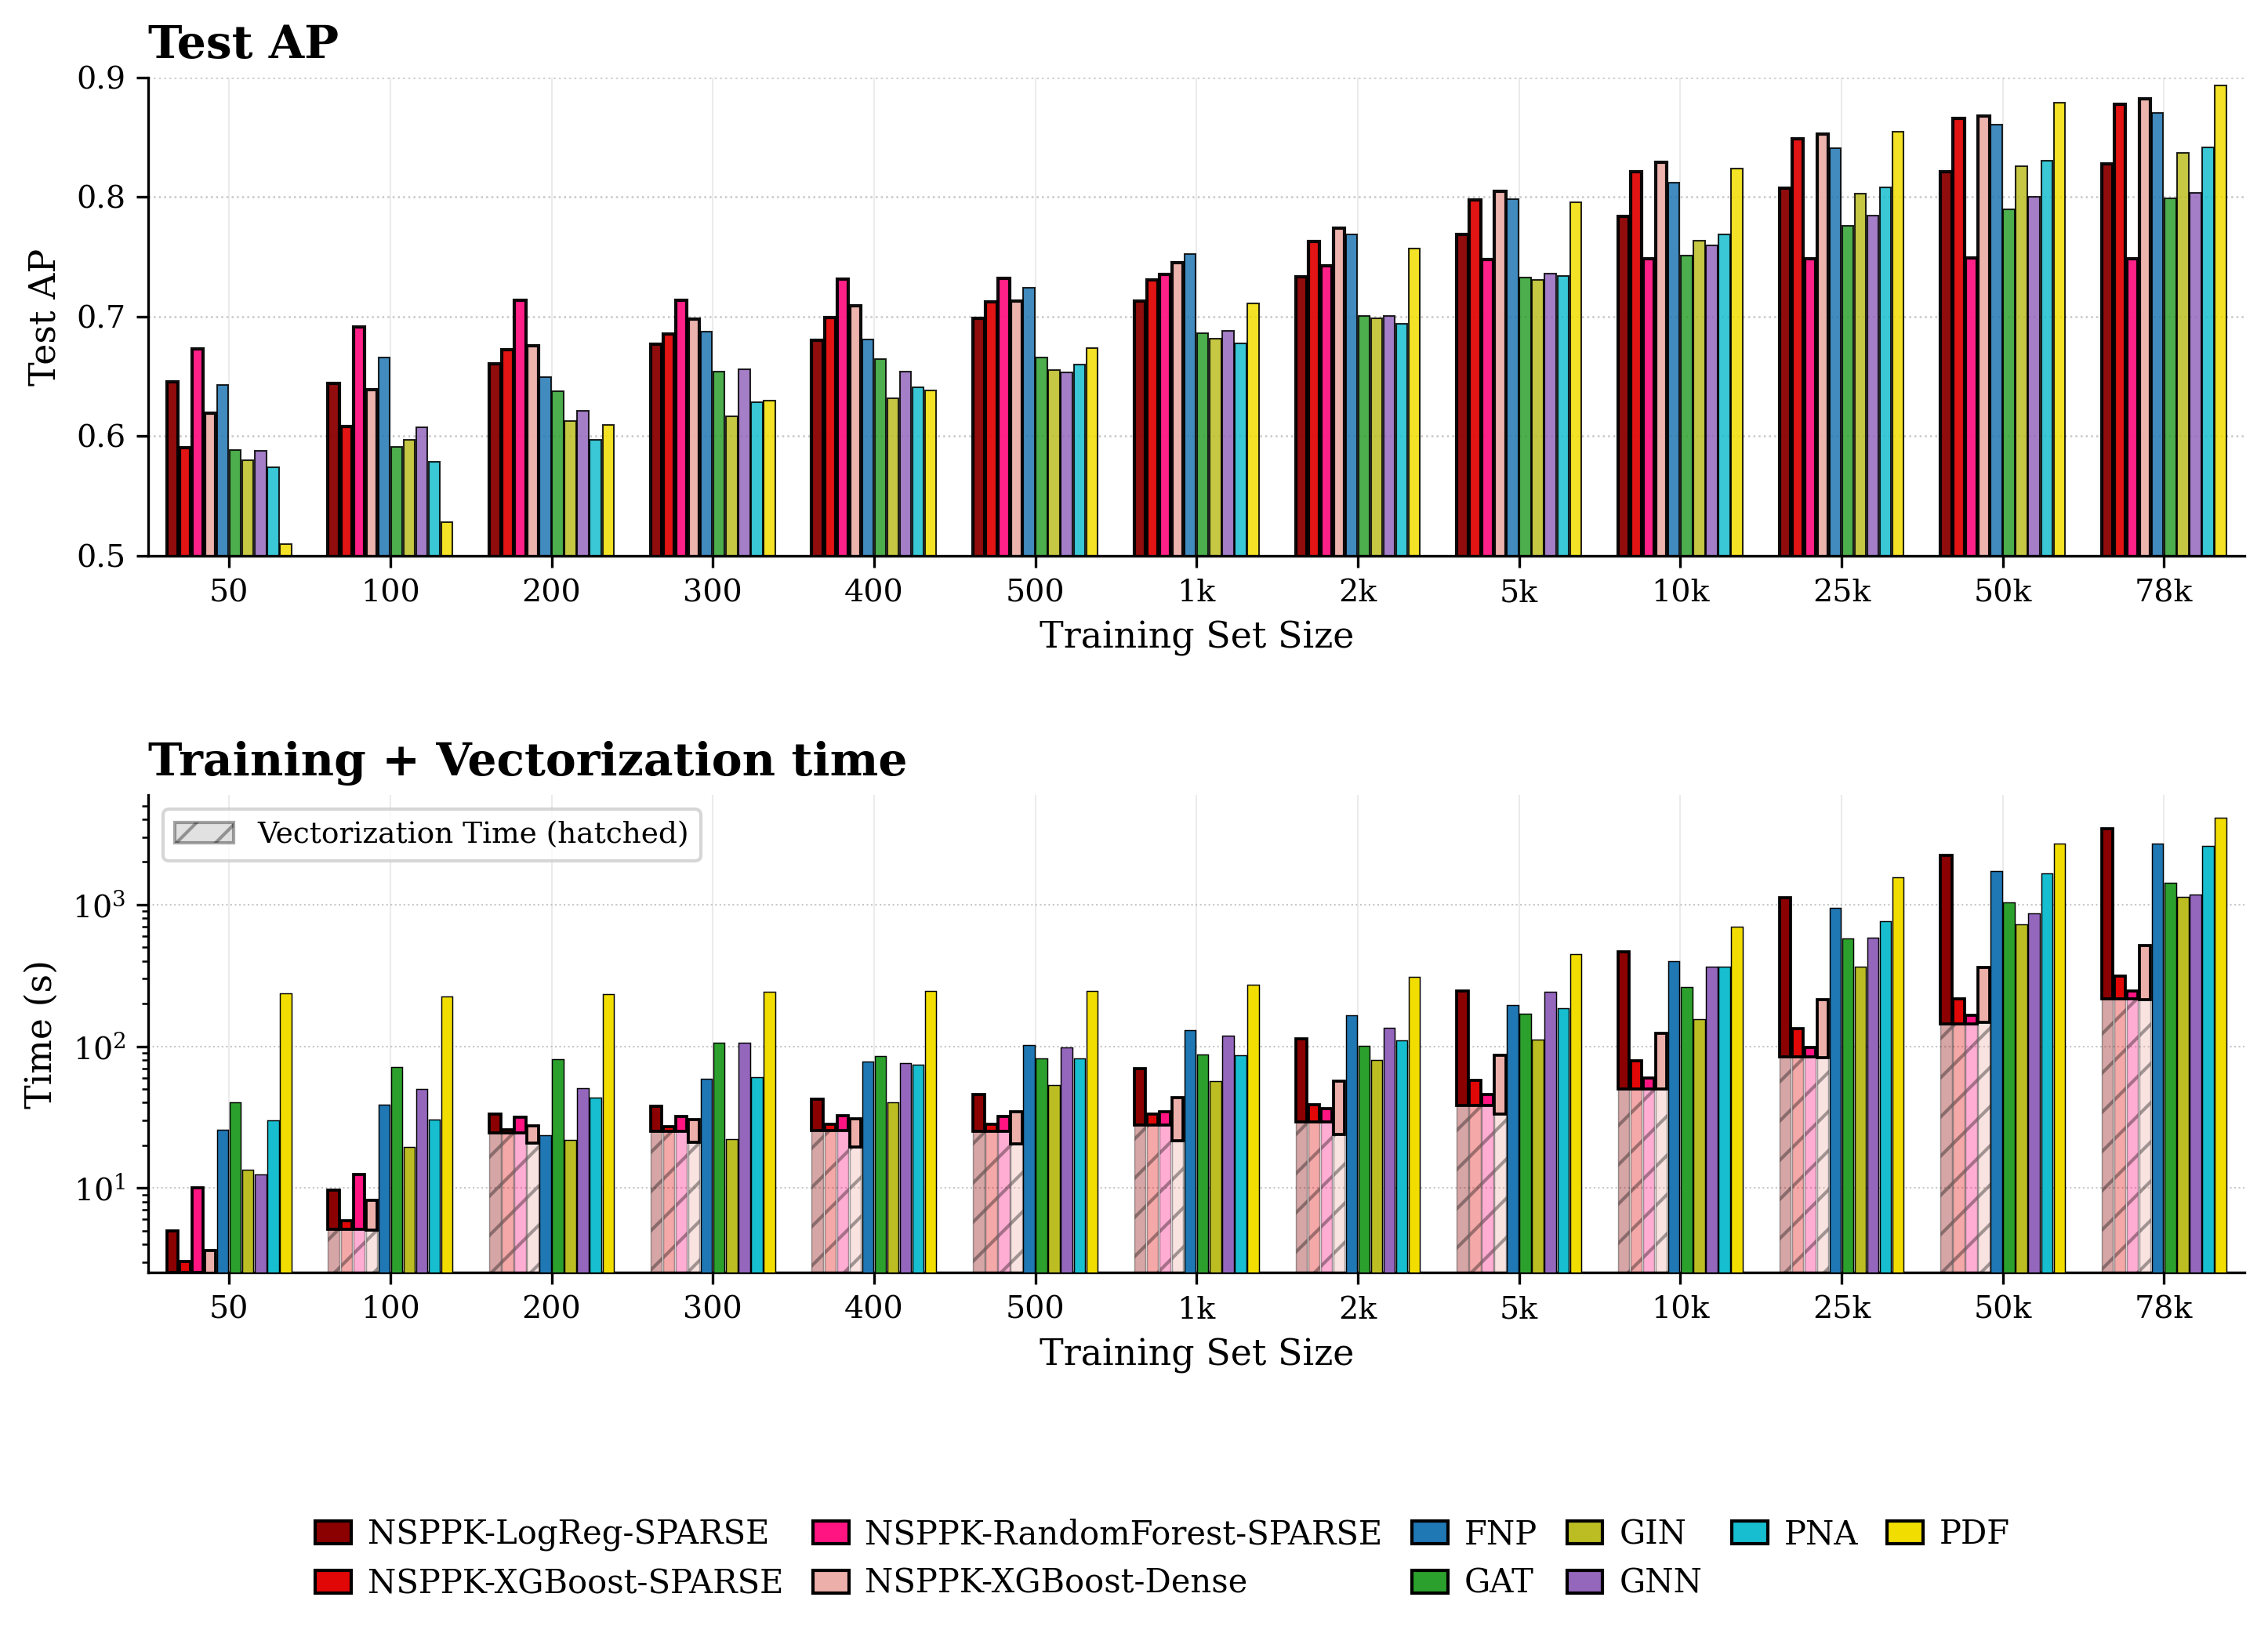
\includegraphics[width=1\textwidth]{images/large_experiment.png}
  \caption{Learning curves on \texttt{ogbg-molpcba} (task 95). NSPPK (red) paired with different downstream classifiers is compared against neural baselines including GIN, GAT, PNA, PDF, and AttentiveFP (FNP).}
  \label{fig:appendix_large_experiment}
\end{figure}

\section{Implementation Details for Task~95 Experiments}
\label{appendix:task95}

\paragraph{NSPPK Configuration.}
For all NSPPK experiments we fixed the parameters across classifiers:
\[
R=1, \quad D=4, \quad R'=1, \quad n_{\text{bits}}=16 .
\]

Both sparse and dense feature representations were evaluated.
Sparse mode stores only non-zero entries and is efficient for CPU-based
models, while dense mode expands the full feature vectors, which can
occasionally benefit GPU-accelerated tree methods.

\paragraph{Downstream Classifiers.}
The exact settings for the classifiers paired with NSPPK features are given in
Table~\ref{tab:nsppk-classifiers}.

\begin{table}[H]
\centering
\caption{Classifiers used with NSPPK features on \texttt{ogbg-molpcba} (task 95).}
\label{tab:nsppk-classifiers}
\begin{tabular}{l l p{7cm}}
\toprule
Classifier & Features & Configuration \\
\midrule
Logistic Regression & Sparse & \texttt{saga}, max\_iter=1000, $L_2$, $n_{\text{jobs}}=64$ \\
Random Forest & Sparse & 500 trees, depth=5, $n_{\text{jobs}}=64$, seed=42 \\
XGBoost & Dense & 1000 trees, depth=6, LR=0.03, subsample=0.8, colsample=0.8 \\
XGBoost & Sparse & Same as above, \texttt{hist} backend \\
\bottomrule
\end{tabular}
\end{table}

\paragraph{Neural Baselines.}
For comparison, we trained common GNN baselines using published
hyperparameters. Table~\ref{tab:nn-baselines} summarizes the main
configurations.

\begin{table}[H]
\centering
\caption{Neural baselines and their configurations for task 95.}
\label{tab:nn-baselines}
\begin{tabular}{l p{7cm} l}
\toprule
Model & Main hyperparameters & Source \\
\midrule
PNA & 2 layers, dim $64\rightarrow32$, batch 64/256, LR=0.001, Adam & \cite{corso2020pna} \\
PDF (Basis-DGL) & 8 layers, dim 384, batch 64/256, LR=$5\times10^{-4}$, AdamW & \cite{yang2023pdf} \\
GAT & 2 layers, dim $64\rightarrow32$, 4/1 heads, LR=0.001, Adam & \cite{velivckovic2018gat} \\
AttentiveFP (FNP) & 4 layers, dim 64, dropout=0.2, LR=0.001, Adam & \cite{xiong2019attentivefp} \\
GIN & 2 layers, dim $64\rightarrow32$, LR=0.001, Adam & \cite{xu2019powerful} \\
GCN (OGB baseline) & 2 layers, dim $64\rightarrow32$, LR=0.001, Adam & \cite{hu2020ogb} \\
\bottomrule
\end{tabular}
\end{table}

\paragraph{Shared Training Setup.}
All neural baselines were trained on the official OGB scaffold split
(train: 249,715; validation: 29,826; test: 29,427).
The loss function was binary cross-entropy with logits
(\texttt{BCEWithLogitsLoss}), and evaluation metrics included AP and ROC--AUC.
Unless otherwise stated, all experiments were executed on CPU.

\paragraph{Reproducibility.}
Balanced-data experiments were repeated with five random seeds.
Both feature extraction time and training time are reported in the main text.

\section{Further Visualization: Accuracy--Time Trade-off}
\label{appendix:tradeoff}

\begin{figure}[H]
\centering
\captionsetup{font=small,aboveskip=3pt,belowskip=0pt}
\captionsetup[subfigure]{font=small}

% ---------- row 1 ----------
\begin{subfigure}[t]{0.32\textwidth}
  \centering
  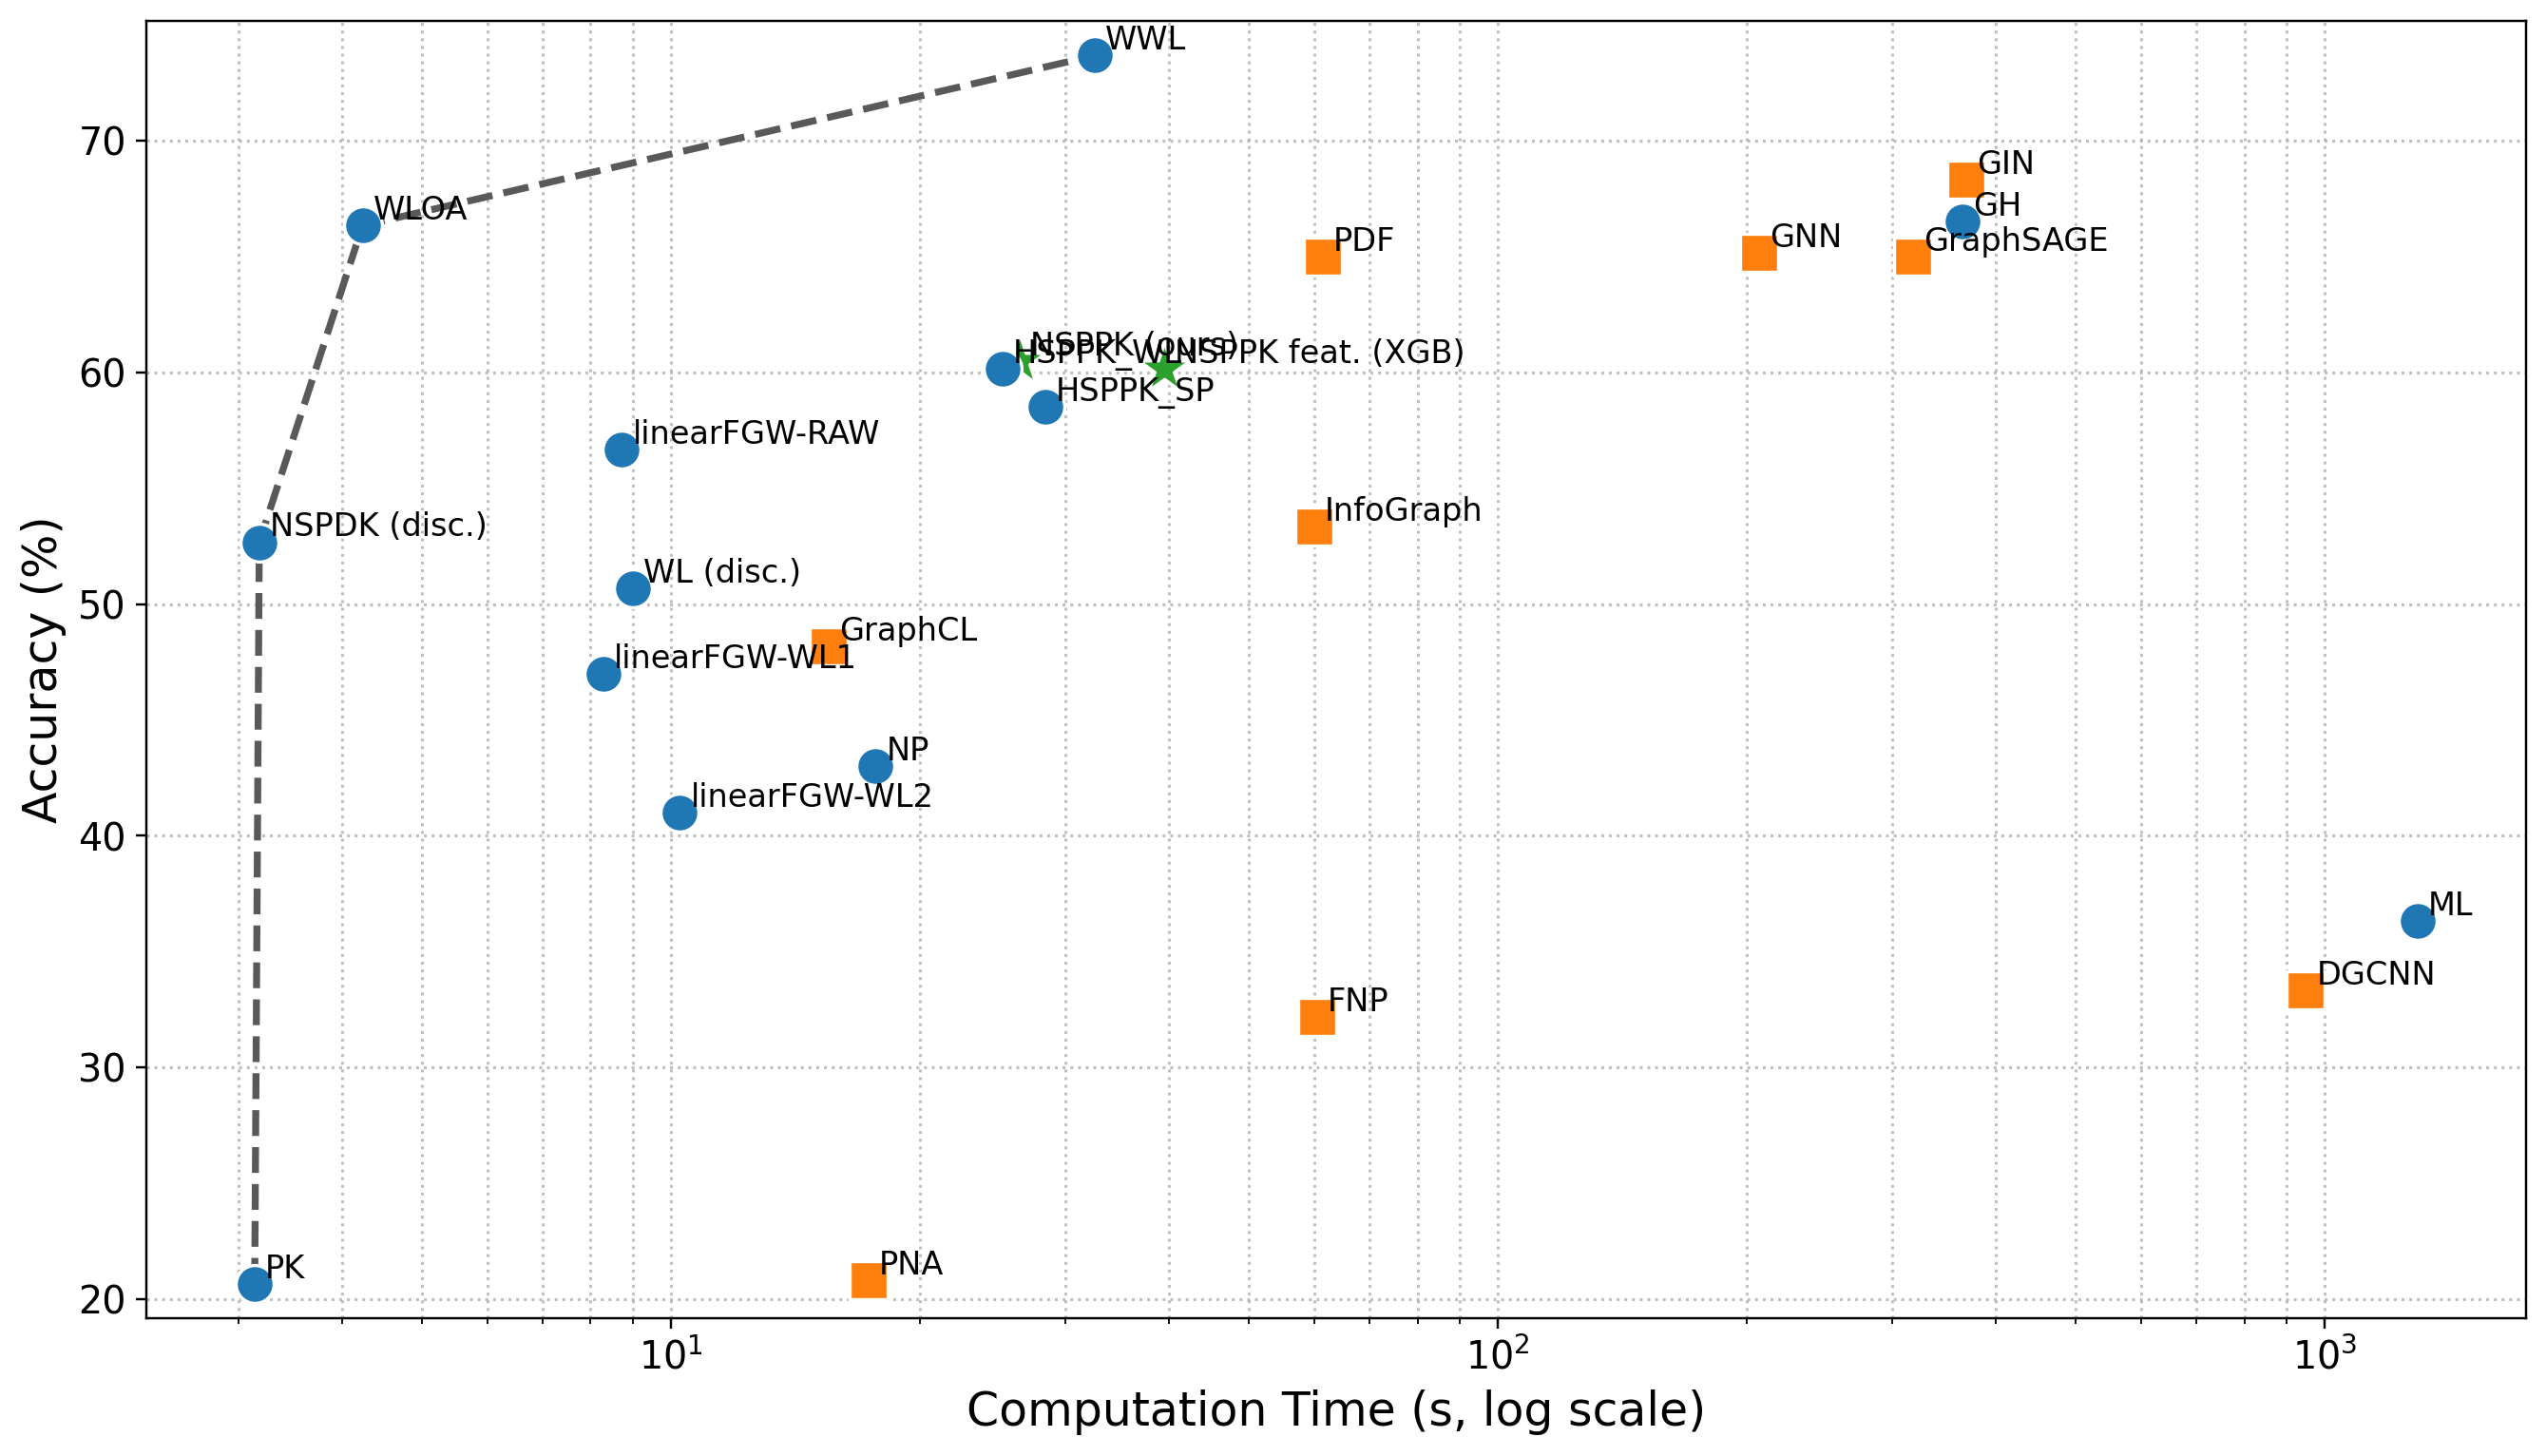
\includegraphics[width=\linewidth]{images/tradeoff_enzymes.png}
  \caption{ENZYMES}
\end{subfigure}\hfill
\begin{subfigure}[t]{0.32\textwidth}
  \centering
  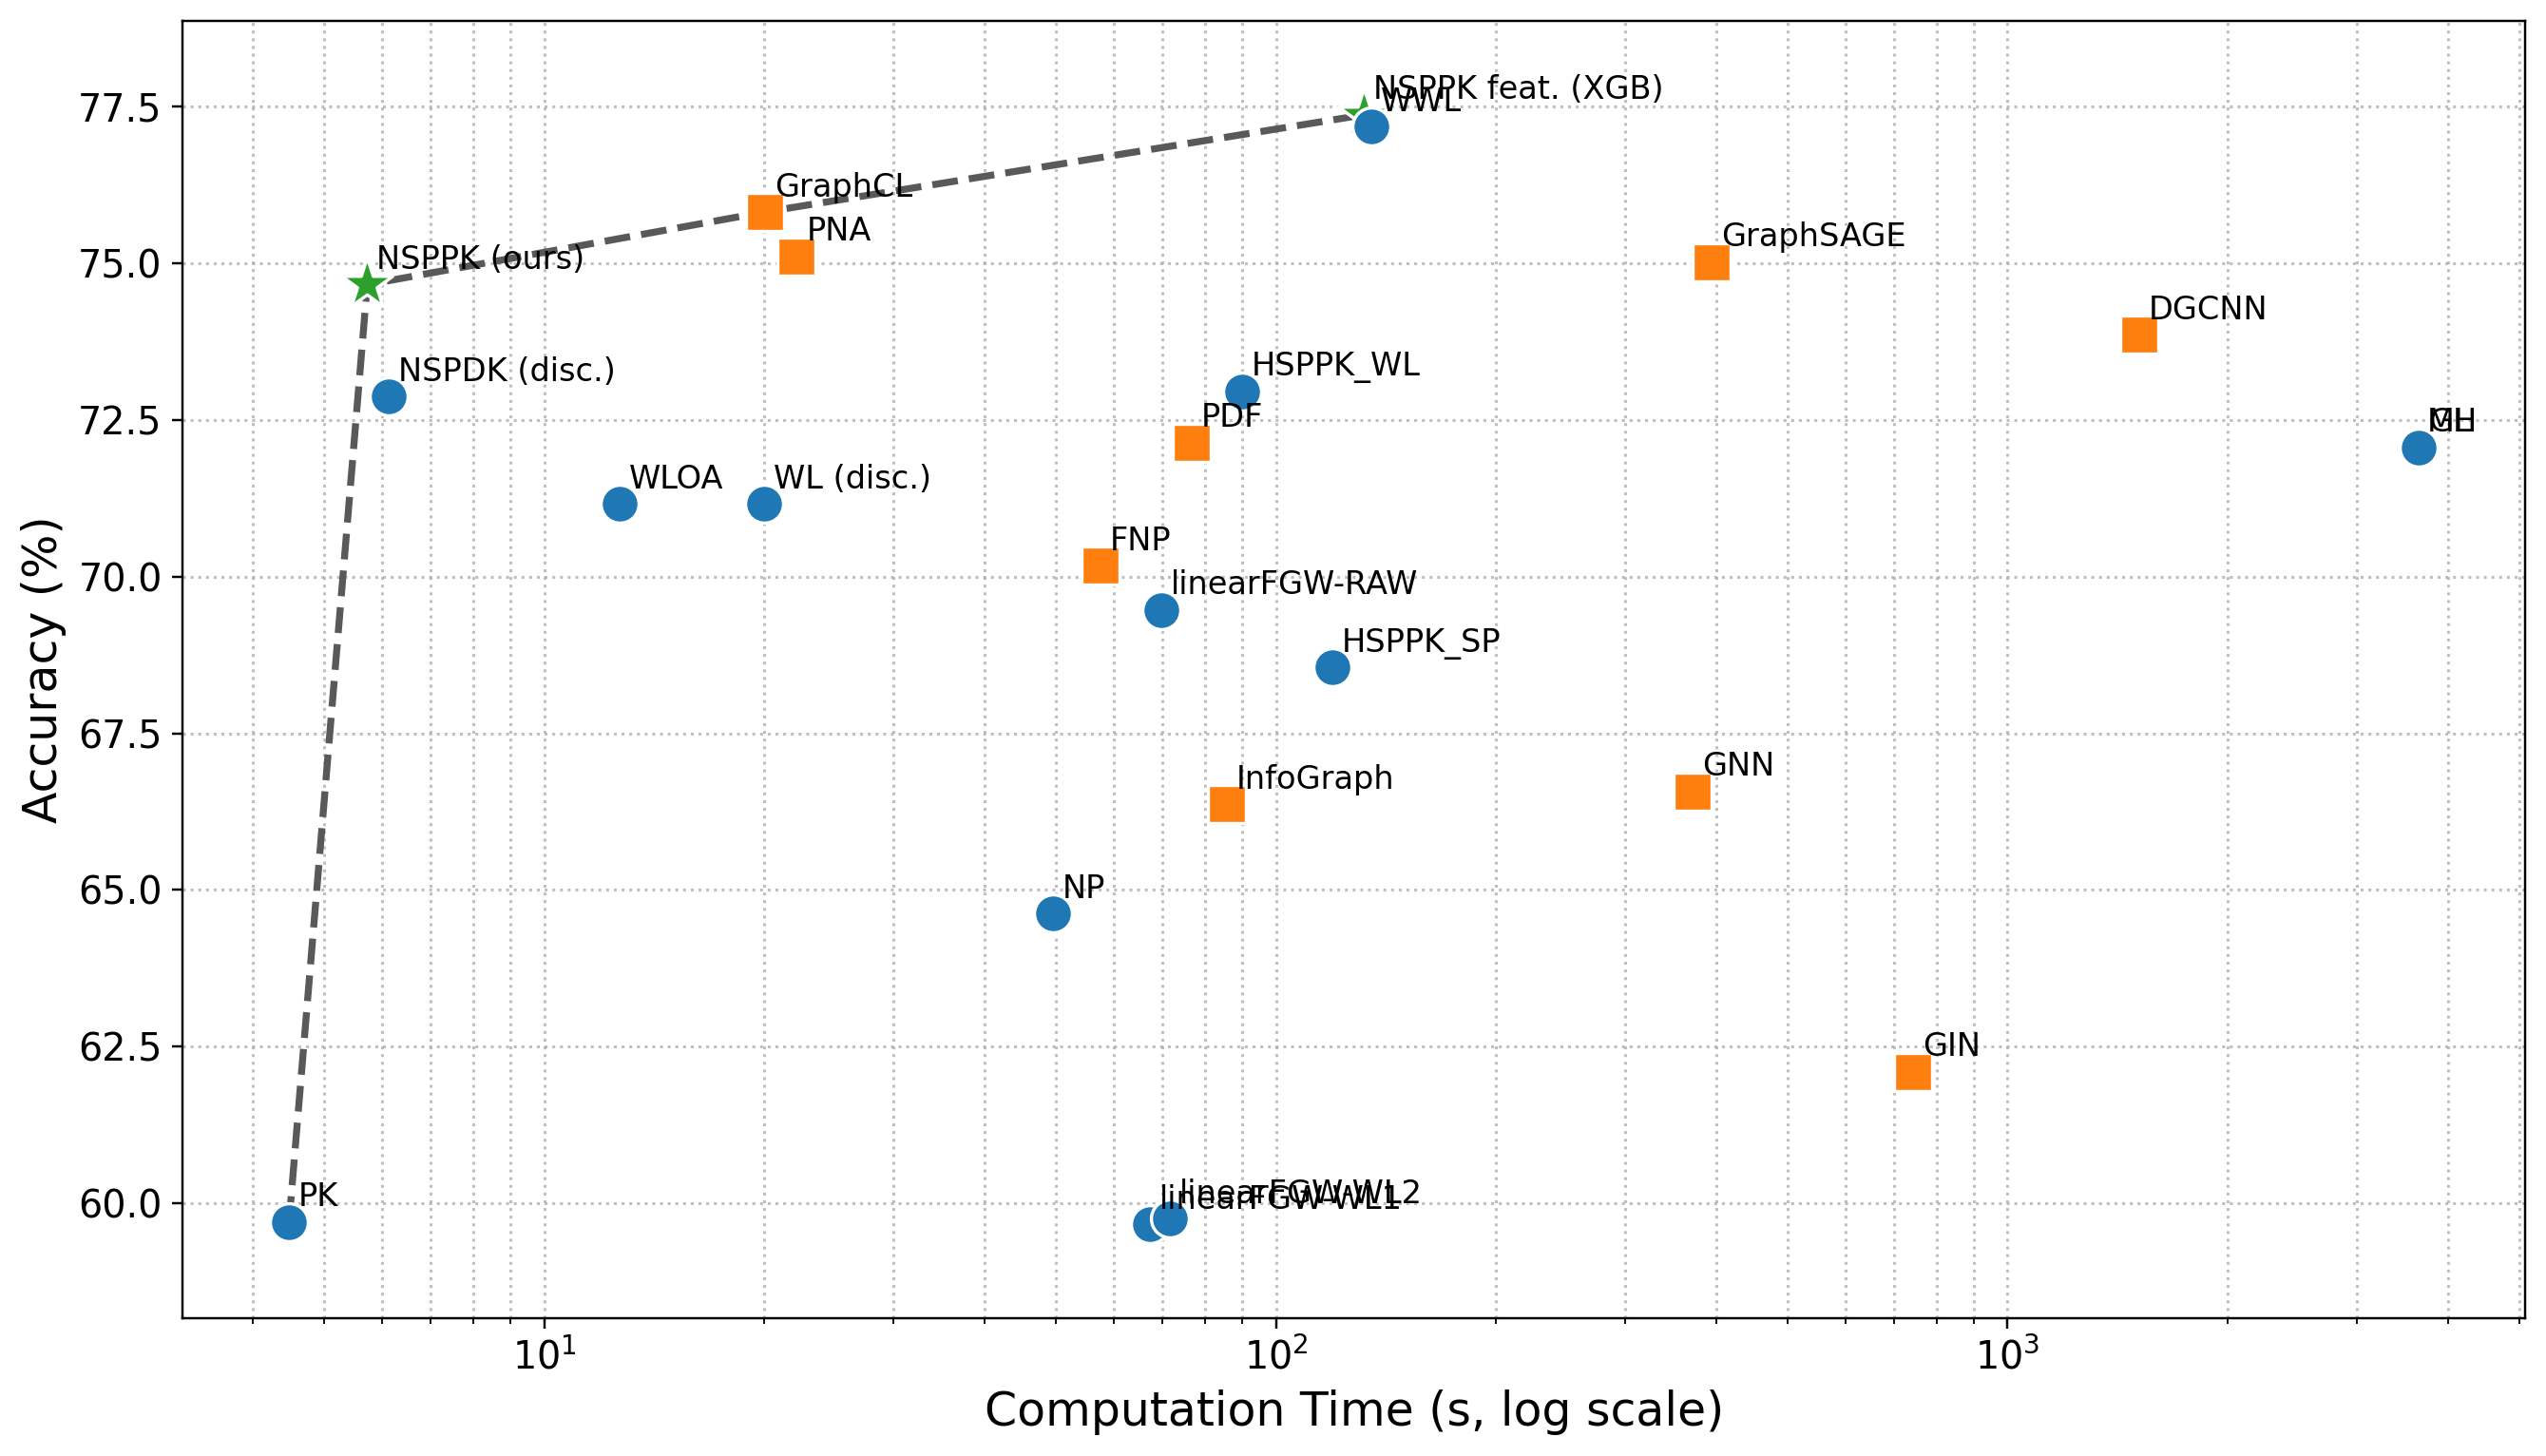
\includegraphics[width=\linewidth]{images/tradeoff_proteins.png}
  \caption{PROTEINS}
\end{subfigure}\hfill
\begin{subfigure}[t]{0.32\textwidth}
  \centering
  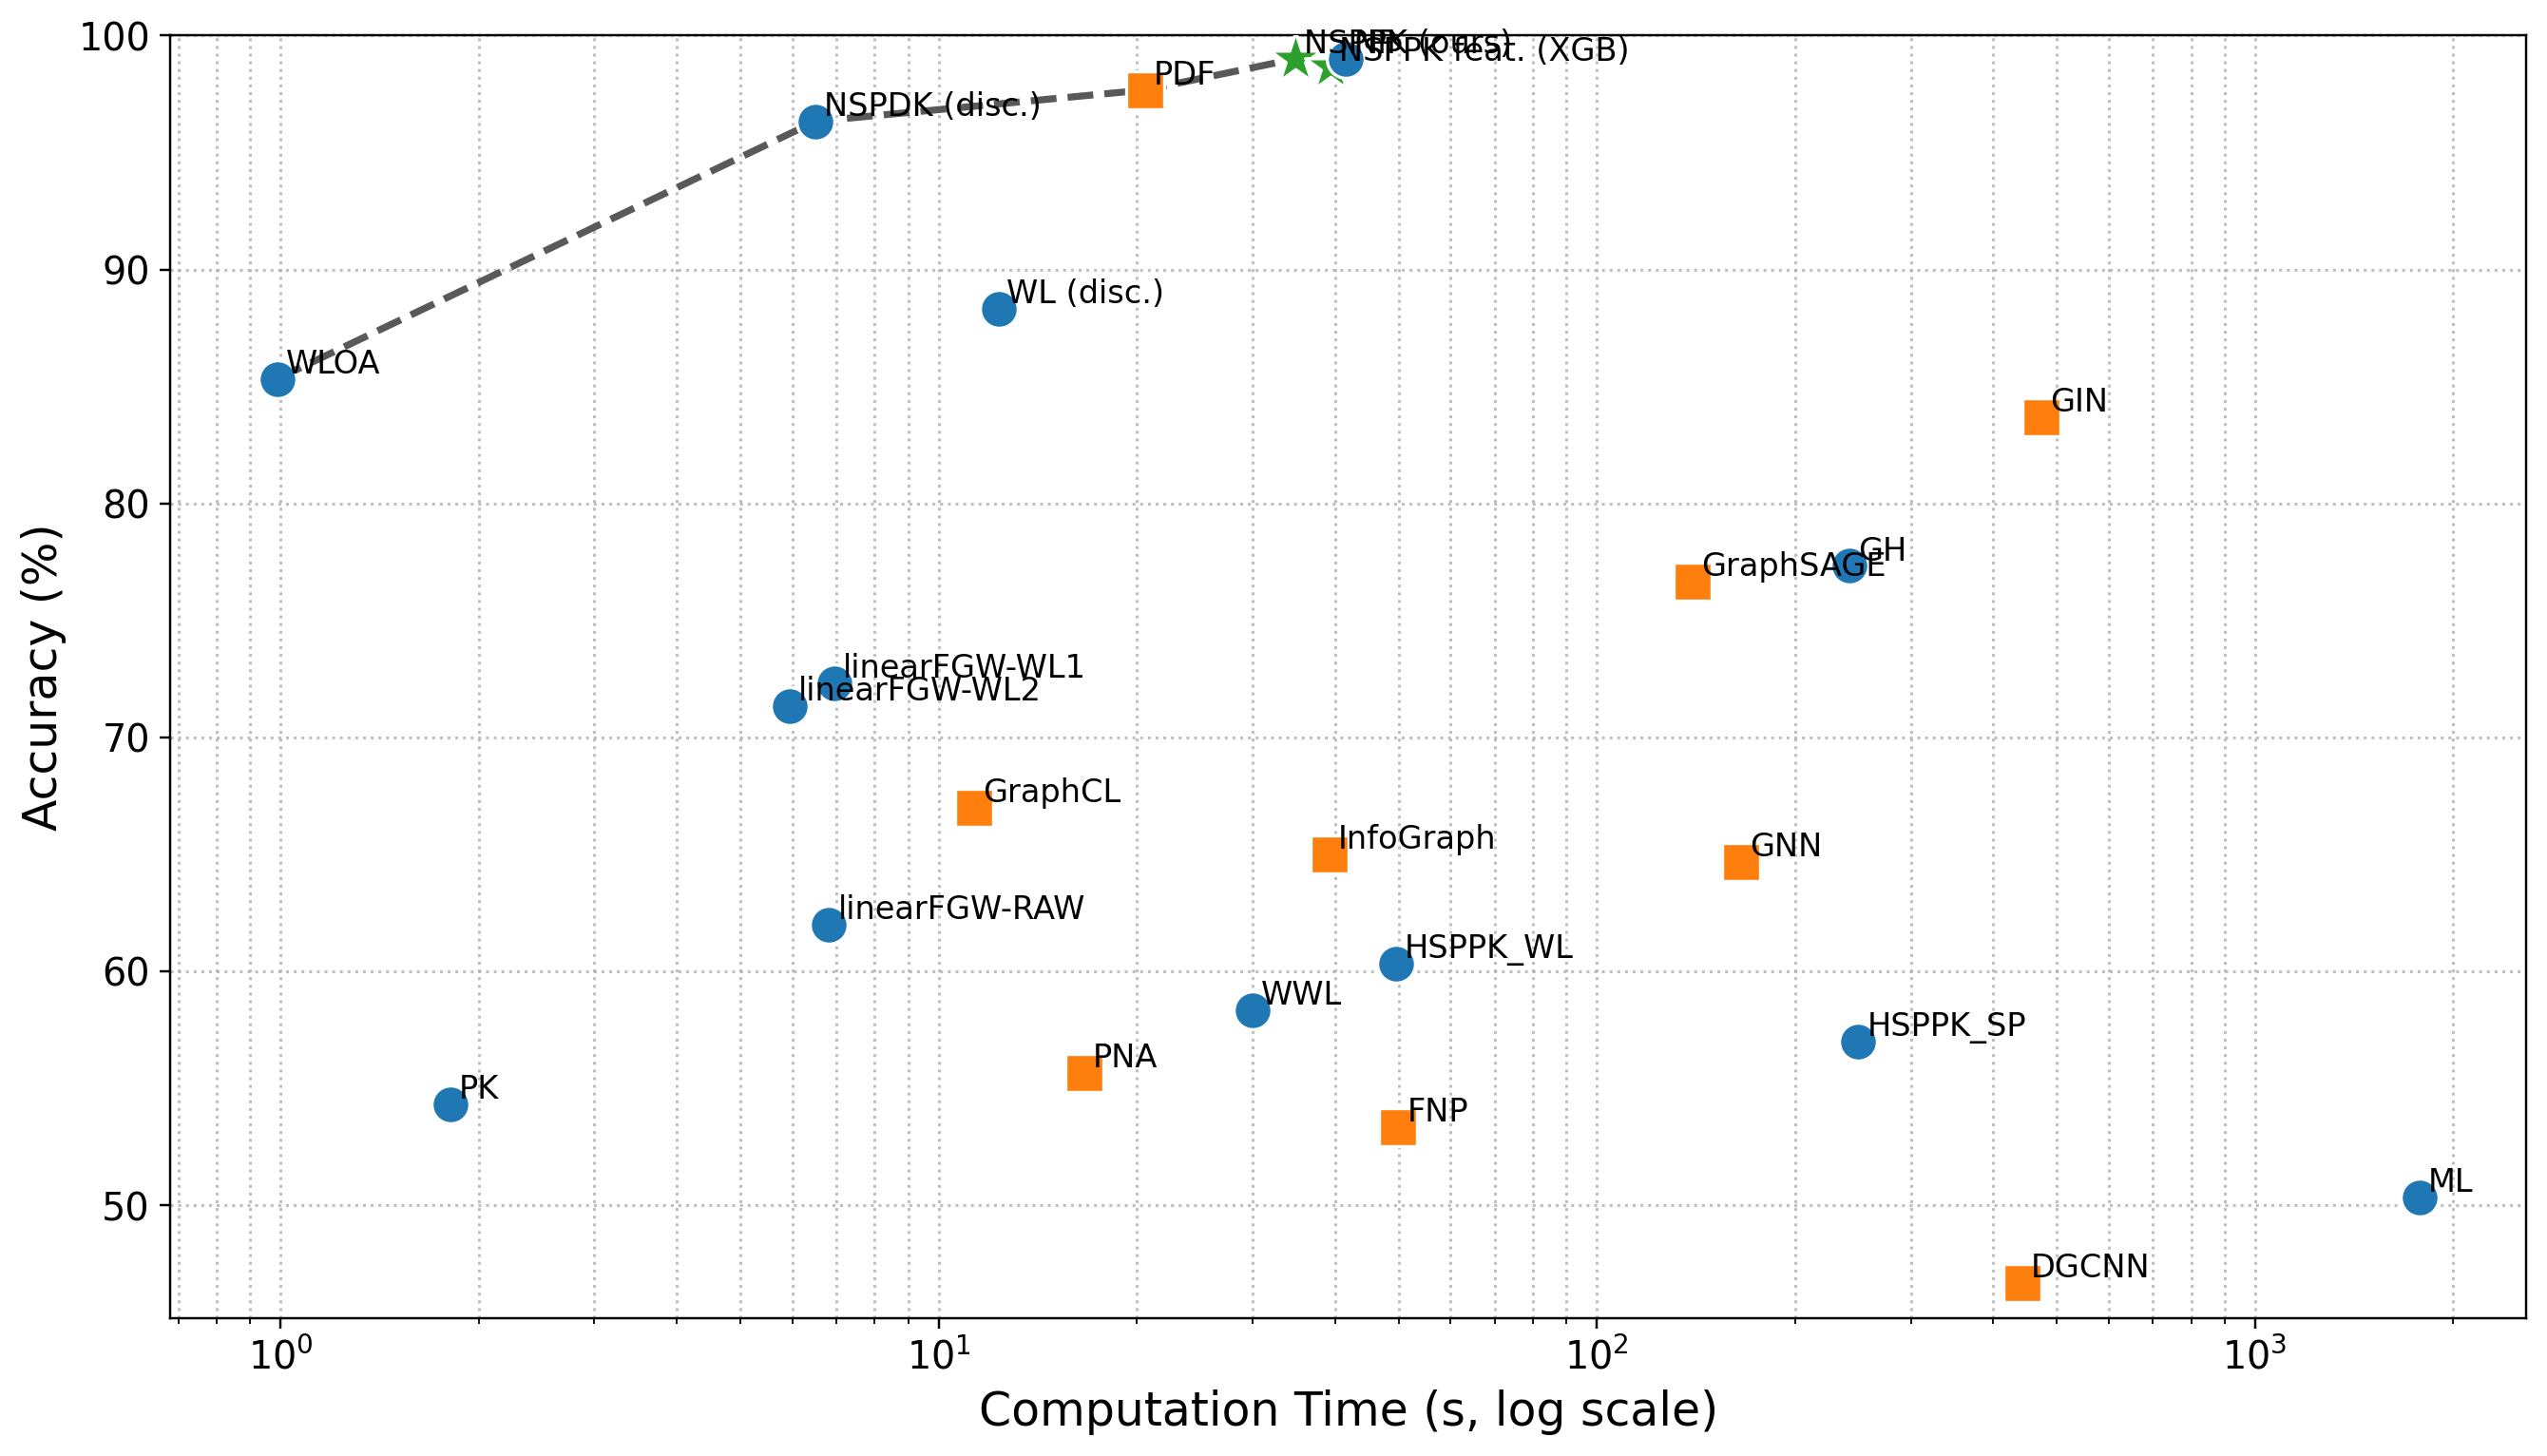
\includegraphics[width=\linewidth]{images/tradeoff_syntheticnew.png}
  \caption{SYNTHETICnew}
\end{subfigure}

\vspace{2pt}

% ---------- row 2 ----------
\begin{subfigure}[t]{0.32\textwidth}
  \centering
  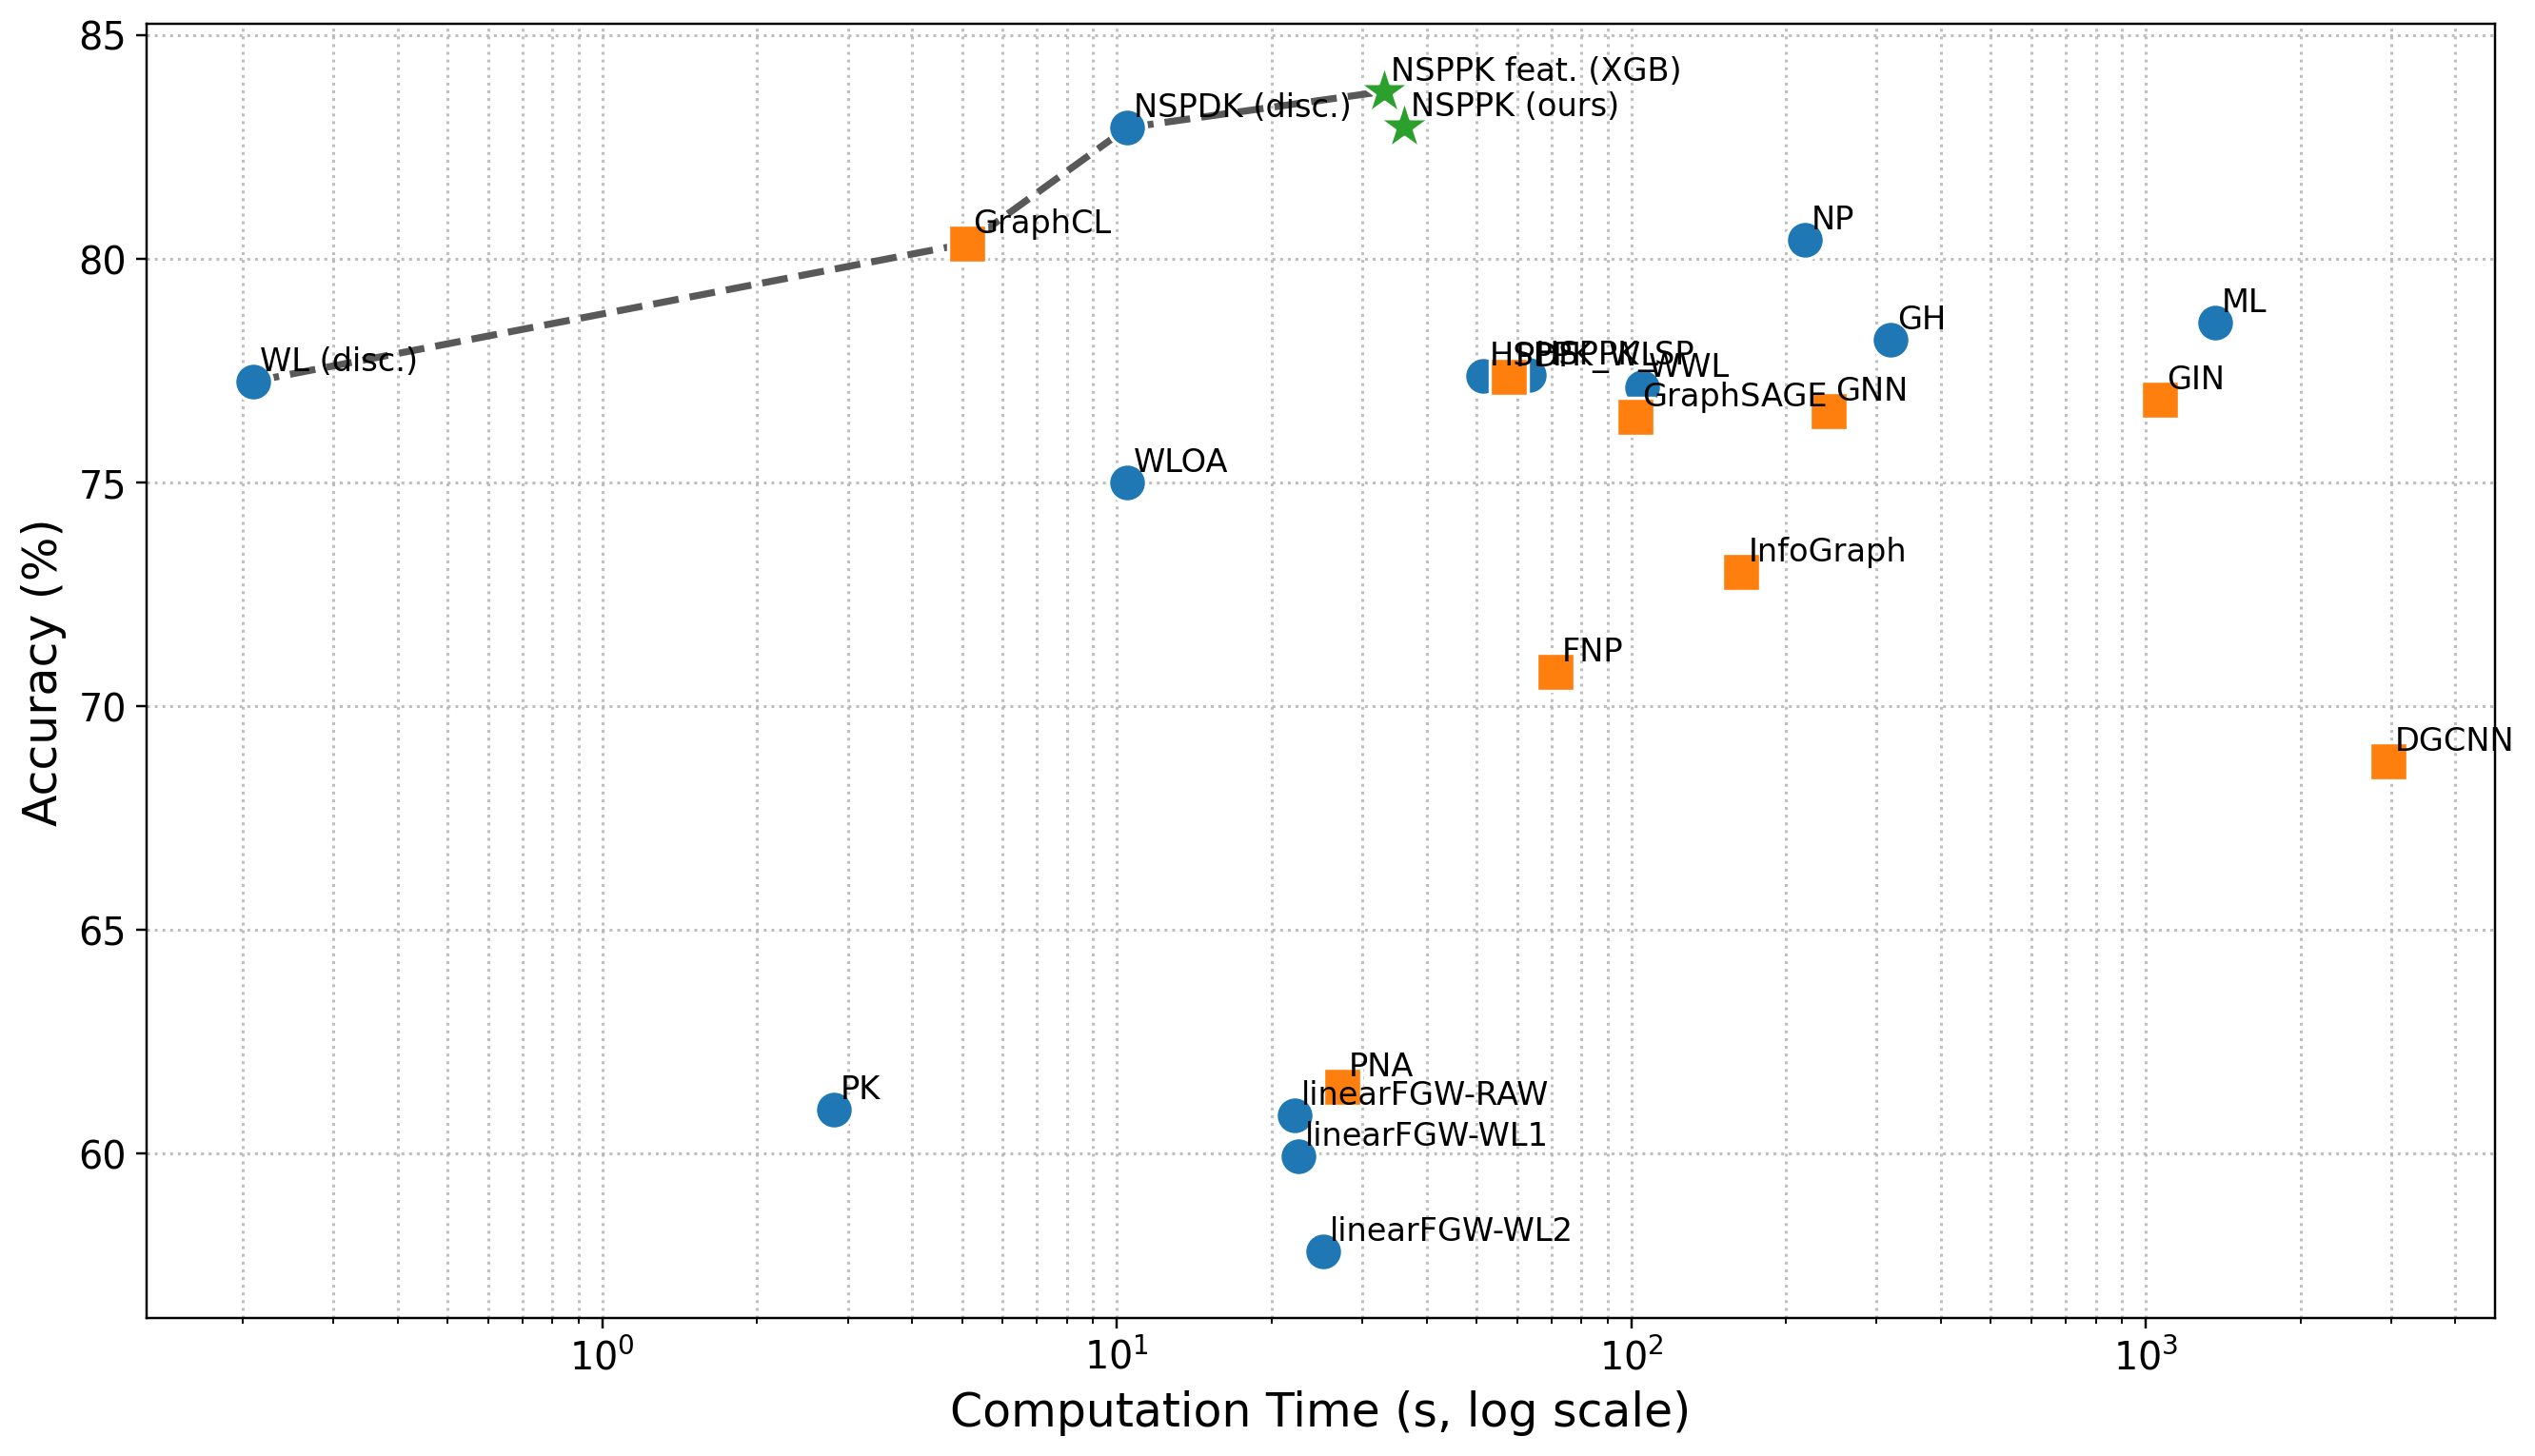
\includegraphics[width=\linewidth]{images/tradeoff_dhfr.png}
  \caption{DHFR}
\end{subfigure}\hfill
\begin{subfigure}[t]{0.32\textwidth}
  \centering
  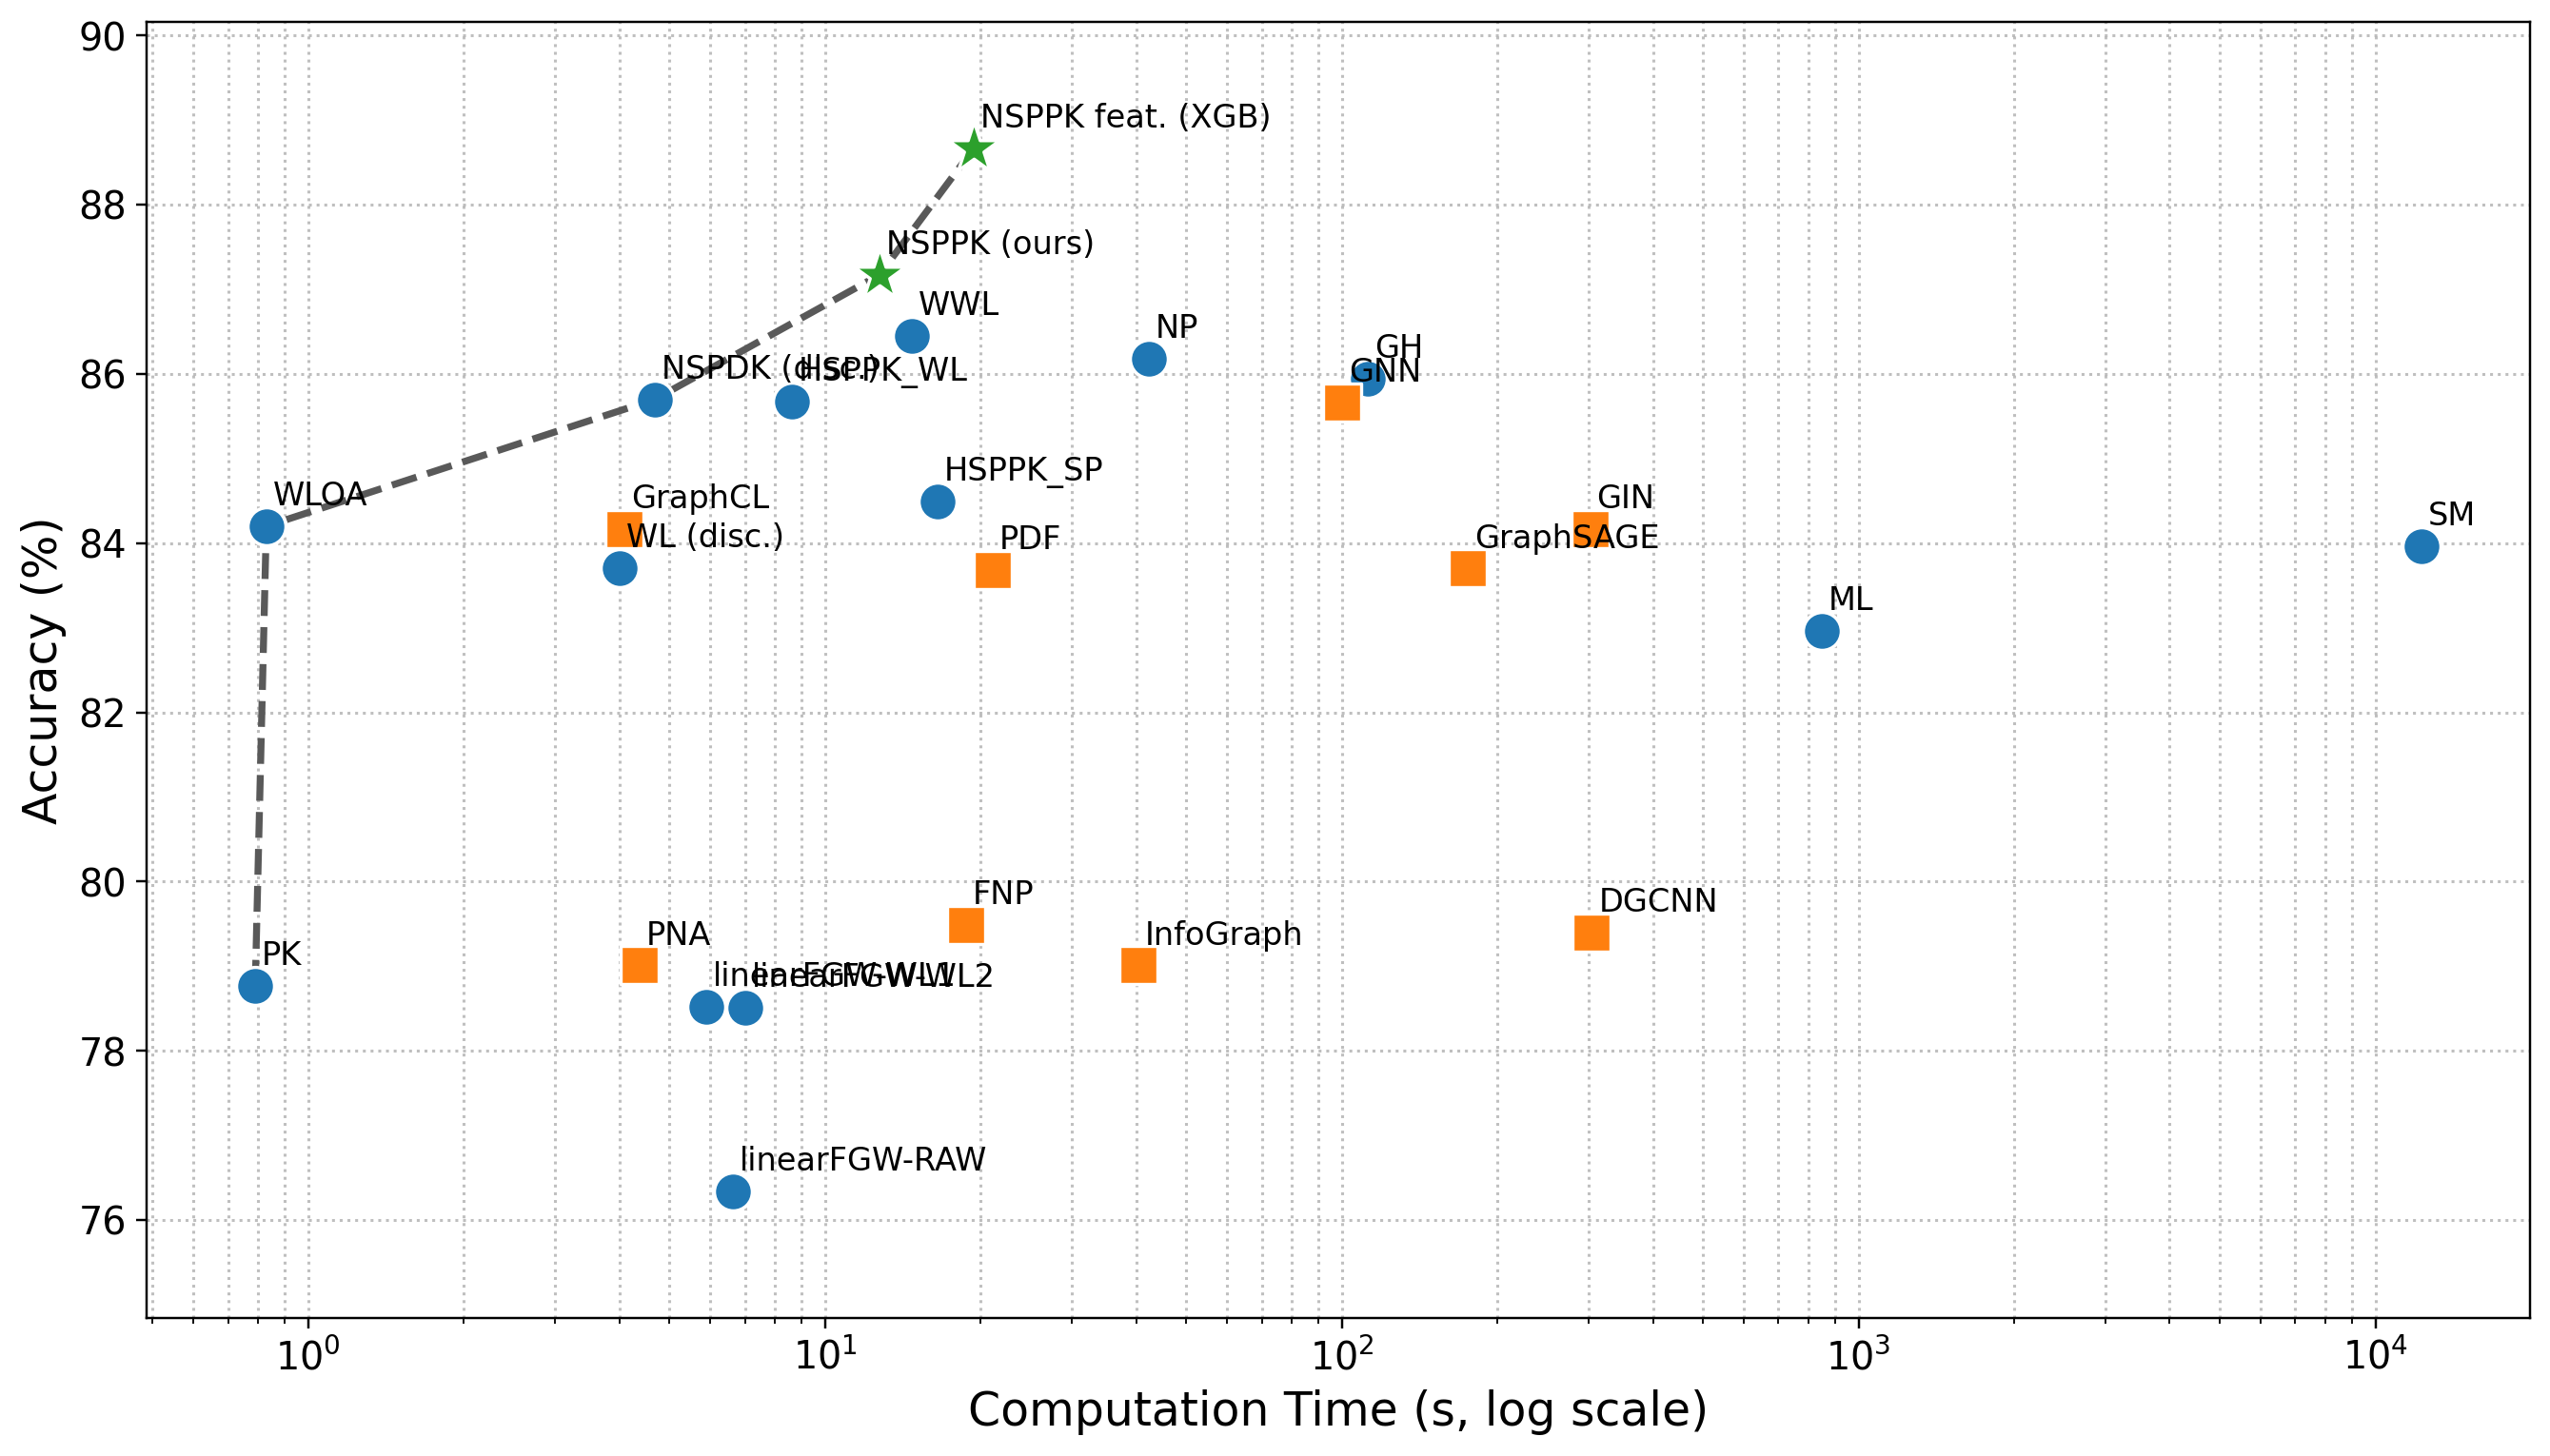
\includegraphics[width=\linewidth]{images/tradeoff_bzr.png}
  \caption{BZR}
\end{subfigure}\hfill
\begin{subfigure}[t]{0.32\textwidth}
  \centering
  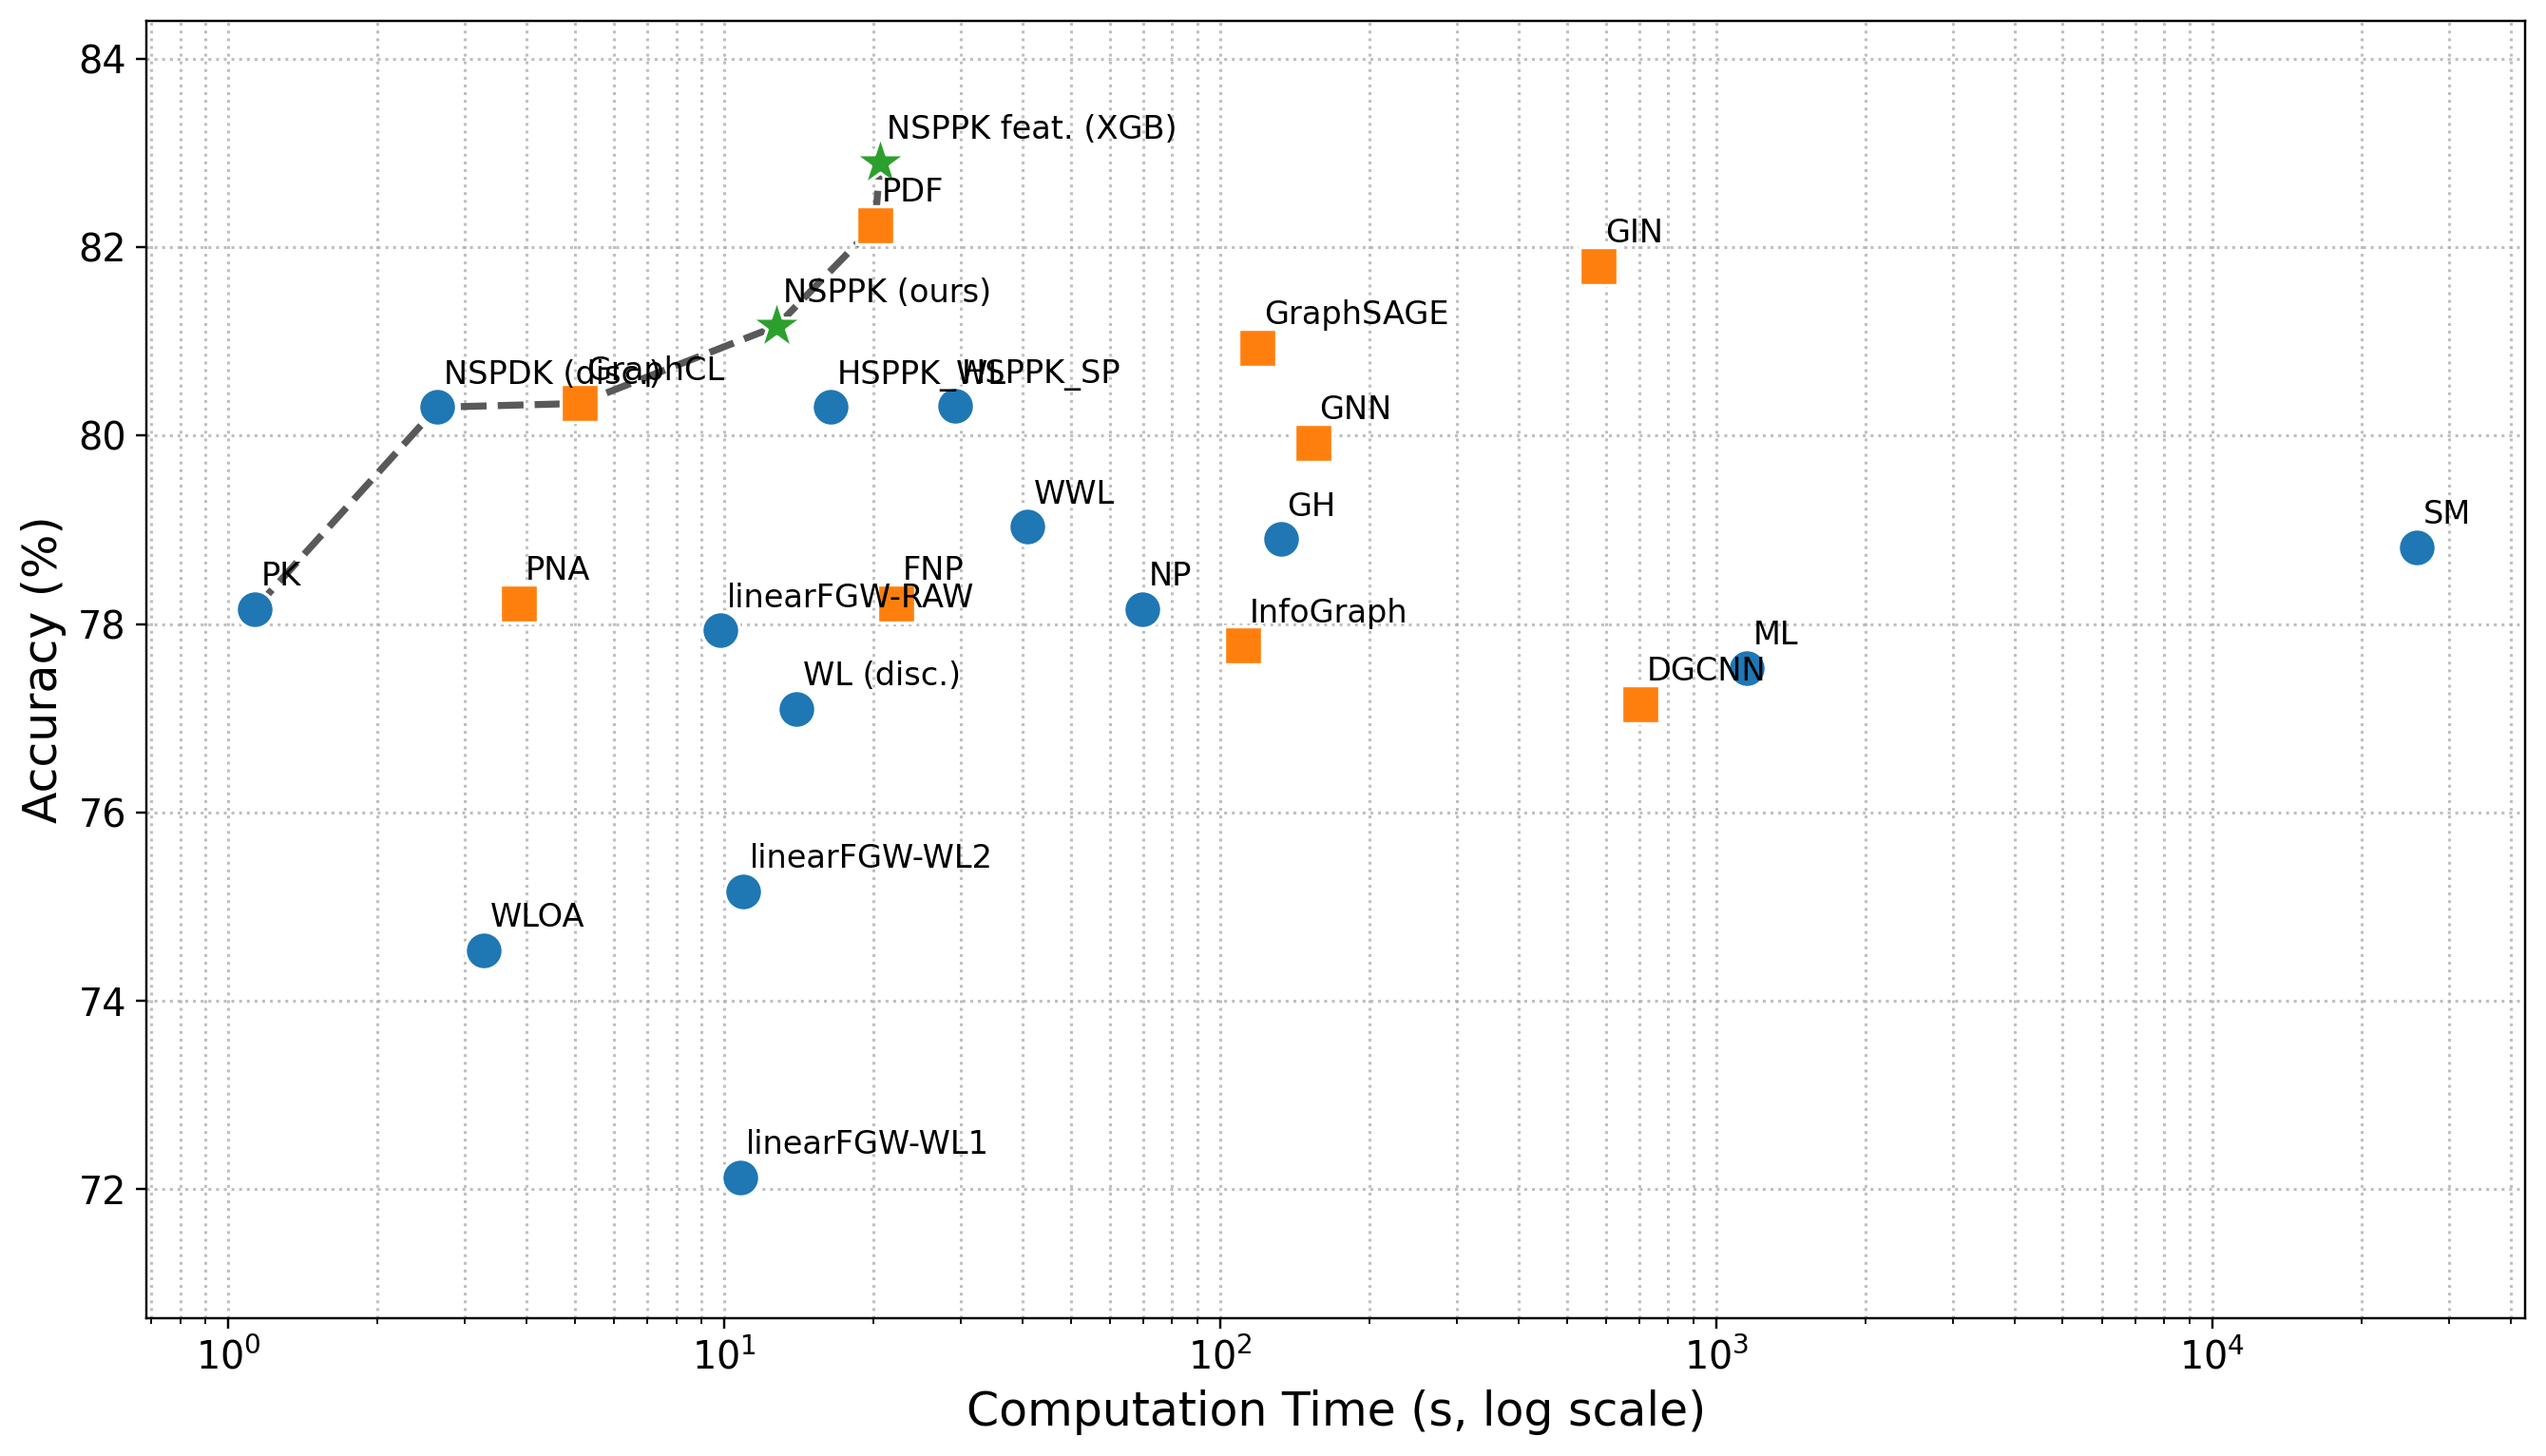
\includegraphics[width=\linewidth]{images/tradeoff_cox2.png}
  \caption{COX2}
\end{subfigure}

\vspace{3pt}

% ---------- bottom (full width) ----------
\begin{subfigure}[t]{0.98\textwidth}
  \centering
  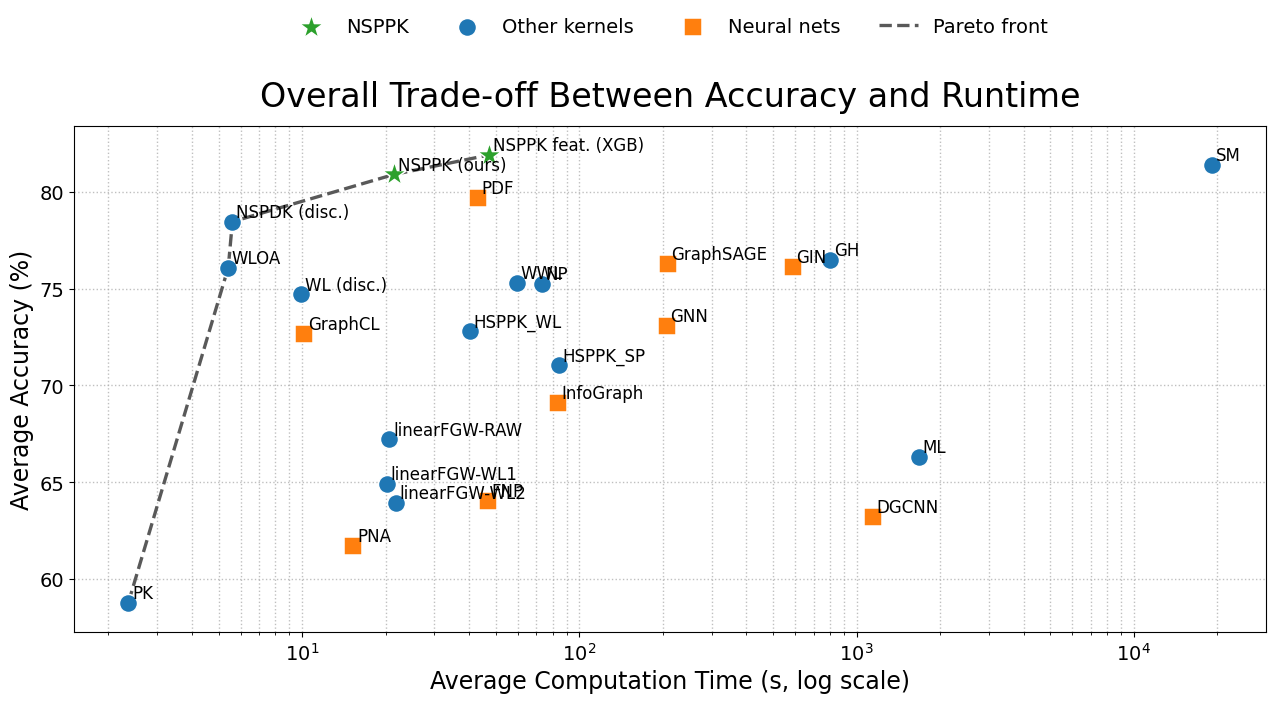
\includegraphics[width=\linewidth]{images/tradeoff_overall_average.png}
  \caption{Overall (average across datasets)}
\end{subfigure}

\caption{\textbf{Accuracy--time trade-off (log runtime).}
Markers denote method families: green star = NSPPK, blue circle = kernel
methods, orange square = neural networks. The dashed line indicates the
Pareto front.}
\label{fig:tradeoff_all}
\end{figure}

\paragraph{Summary.}
Figure~\ref{fig:tradeoff_all} shows that, for most datasets, NSPPK
(green star) lies on or close to the Pareto frontier. Methods are distributed
along the efficiency--accuracy spectrum: some are faster but less accurate,
while others achieve slightly higher accuracy at significantly greater
computational cost. In the aggregated panel, NSPPK remains on the global
frontier, indicating a favourable balance between predictive performance and
runtime.

\section{Additional Results in the No-Attribute Setting}
\label{appendix:no_attr}

To isolate the structural contribution of each method, we repeated the
graph classification experiments after removing all node attributes.
Tables~\ref{tab:no_attr} and~\ref{tab:nn_no_attr} report the resulting
classification accuracies for kernel and neural methods, respectively.
Overall, NSPPK remains competitive in this structural-only setting,
indicating that its performance does not depend solely on attribute
information and that it captures meaningful structural regularities.

% ========================= WITHOUT ATTRIBUTES =========================
\begin{table}[H]
\centering
\caption{Classification accuracy (\%) \textbf{without} node attributes, with average rank.}
\label{tab:no_attr}
\scriptsize
\setlength{\tabcolsep}{3.2pt}
\begin{adjustbox}{max width=\textwidth}
\begin{tabular}{lccccccc}
\toprule
\textbf{Method} & \makecell{SYNTHETIC\\new} & \textbf{DHFR} & \textbf{BZR} & \textbf{COX2} & \textbf{ENZYMES} & \textbf{PROTEINS} & \textbf{Avg Rank} \\
\midrule
SM  & \TO & \TO & \mps{79.02}{1.10} & \mps{78.16}{0.81} & \TO & \TO & 8.75 \\
SP  & \TO & \TO & \TO & \TO & \TO & \TO & -- \\
ML  & \mps{67.22}{9.51} & \mps{79.90}{1.36} & \mps{86.63}{3.81} & \mps{77.95}{4.63} & \mps{33.66}{5.31} & \mps{72.80}{3.80} & \textbf{4.17} \\
PK  & \mps{61.33}{7.33} & \mps{60.98}{0.48} & \mps{78.77}{1.01} & \mps{78.16}{8.07} & \mps{18.33}{5.22} & \mps{58.48}{4.29} & 10.83 \\
HSPPK\_WL & \mps{50.00}{0.00} & \mps{57.56}{6.67} & \mps{80.26}{3.02} & \mps{72.41}{17.06} & \mps{16.50}{2.73} & \mps{63.80}{5.76} & 11.17 \\
HSPPK\_SP & \mps{58.00}{7.18} & \mps{64.42}{4.05} & \mps{76.26}{9.39} & \mps{77.31}{4.70} & \mps{21.00}{5.92} & \mps{46.20}{4.70} & 11.67 \\
GH  & \mps{59.33}{9.28} & \mps{74.08}{4.27} & \mps{81.25}{2.40} & \mps{77.30}{3.14} & \mps{25.17}{3.98} & \mps{71.61}{4.32} & 7.17 \\
NP  & \mps{97.00}{3.15} & \mps{80.43}{4.01} & \mps{84.16}{5.65} & \mps{80.29}{3.42} & \mps{36.70}{0.53} & \mps{69.99}{3.88} & 5.17 \\
linearFGW-RAW & \mps{57.33}{6.29} & \mps{54.90}{4.77} & \mps{80.52}{3.76} & \mps{76.24}{4.74} & \mps{23.00}{4.88} & \mps{71.35}{4.56} & 8.33 \\
linearFGW-WL1 & \mps{56.00}{11.72} & \mps{63.90}{3.97} & \mps{80.99}{5.24} & \mps{76.45}{1.86} & \mps{24.50}{4.78} & \mps{70.17}{4.81} & 8.17 \\
linearFGW-WL2 & \mps{48.67}{7.33} & \mps{59.12}{6.41} & \mps{79.48}{5.48} & \mps{74.74}{5.12} & \mps{22.33}{5.59} & \mps{69.54}{3.12} & 9.50 \\
WL (disc.) & \mps{79.00}{12.39} & \mps{80.56}{5.29} & \mps{87.90}{3.92} & \mps{78.17}{3.48} & \mps{40.17}{7.54} & \mps{69.00}{4.08} & \textbf{3.83} \\
WLOA & \mps{81.00}{6.16} & \mps{80.96}{3.90} & \mps{83.71}{8.36} & \mps{78.16}{2.75} & \mps{42.67}{4.84} & \mps{74.49}{3.53} & 4.67 \\
WWL & \mps{50.00}{0.00} & \mps{60.98}{0.47} & \mps{78.77}{1.01} & \mps{78.16}{0.80} & \mps{16.67}{0.00} & \mps{55.57}{0.17} & 12.17 \\
NSPDK & \mps{95.33}{3.72} & \mps{82.94}{5.70} & \mps{85.68}{4.04} & \mps{77.09}{3.84} & \mps{35.67}{9.22} & \mps{71.33}{3.06} & 6.00 \\
NSPDK (disc.) & \mps{95.33}{3.72} & \mps{82.94}{5.70} & \mps{85.68}{4.04} & \mps{77.09}{3.84} & \mps{35.67}{9.22} & \mps{71.33}{3.06} & 6.00 \\
\rowcolor{gray!10}
\textbf{NSPPK (ours)} & \mps{98.00}{3.93} & \mps{80.18}{5.58} & \mps{87.65}{4.54} & \mps{77.73}{3.96} & \mps{33.17}{5.80} & \mps{71.34}{4.06} & \textbf{4.33} \\
\bottomrule
\end{tabular}
\end{adjustbox}

\vspace{0.5ex}
\footnotesize\emph{Note:} Average rank is computed over available entries only; lower is better. Timeouts and unavailable results are omitted on a per-dataset basis.
\end{table}

% ========================= NEURAL NETS — WITHOUT ATTRIBUTES =========================
\begin{table}[H]
\centering
\caption{Neural network classification accuracy (\%) \textbf{without} node attributes, with average rank.}
\label{tab:nn_no_attr}
\scriptsize
\setlength{\tabcolsep}{3.2pt}
\begin{adjustbox}{max width=\textwidth}
\begin{tabular}{lccccccc}
\toprule
\textbf{Method} &
\makecell{SYNTHETIC\\new} &
\textbf{DHFR} &
\textbf{BZR} &
\textbf{COX2} &
\textbf{ENZYMES} &
\textbf{PROTEINS} &
\textbf{Avg Rank} \\
\midrule
DGCNN     & \mps{44.67}{6.86} & \mps{61.50}{4.93} & \mps{81.98}{2.20} & \mps{78.22}{0.07} & \mps{26.80}{7.09} & \mps{73.22}{3.48} & 6.83 \\
GraphSAGE & \mps{43.33}{5.58} & \mps{78.06}{6.25} & \mps{83.70}{5.59} & \mps{80.30}{0.03} & \mps{48.17}{7.58} & \mps{74.93}{2.82} & 4.83 \\
InfoGraph & \mps{67.33}{21.54} & \mps{71.53}{8.51} & \mps{75.05}{15.04} & \mps{69.02}{0.20} & \mps{53.33}{4.79} & \mps{63.07}{4.69} & 5.50 \\
GIN       & \mps{53.00}{9.71} & \mps{79.91}{7.91} & \mps{73.95}{3.30} & \mps{79.91}{0.08} & \mps{42.67}{7.68} & \mps{65.77}{5.02} & 5.17 \\
GraphCL   & \mps{50.00}{8.69} & \mps{80.16}{2.51} & \mps{79.99}{3.62} & \mps{81.38}{3.79} & \mps{37.50}{5.12} & \mps{71.43}{3.92} & 4.00 \\
GNN       & \mps{43.33}{5.58} & \mps{82.67}{4.96} & \mps{84.66}{4.60} & \mps{81.60}{5.54} & \mps{48.50}{5.80} & \mps{71.79}{3.61} & 4.17 \\
FNP       & \mps{50.00}{8.69} & \mps{60.85}{4.63} & \mps{81.73}{3.52} & \mps{78.22}{3.94} & \mps{35.83}{7.79} & \mps{72.41}{3.70} & 5.00 \\
PNA       & \mps{46.00}{7.72} & \mps{60.98}{4.46} & \mps{78.76}{4.33} & \mps{78.22}{7.01} & \mps{18.83}{7.07} & \mps{70.62}{3.69} & 7.50 \\
PDF       & \mps{50.00}{8.69} & \mps{78.83}{4.21} & \mps{84.43}{4.63} & \mps{81.38}{3.79} & \mps{52.00}{5.26} & \mps{74.75}{2.28} & 3.67 \\
\rowcolor{gray!10}
NSPPK feat.\ (XGBoost)
          & \mps{91.00}{4.73} & \mps{78.44}{1.27} & \mps{89.60}{3.29} & \mps{82.76}{4.25} & \mps{41.83}{5.55} & \mps{71.60}{3.15} & \textbf{2.33} \\
\bottomrule
\end{tabular}
\end{adjustbox}
\end{table}

\section{Additional Runtime Results in the No-Attribute Setting}
\label{appendix:no_attr_runtime}

Tables~\ref{tab:no_attr_runtime_kernels} and~\ref{tab:no_attr_runtime_nns}
report computation times in the no-attribute setting for kernel and neural
methods, respectively. As expected, runtimes are generally lower once node
attributes are removed. Nevertheless, the relative efficiency trends remain
similar to those observed in the attributed setting, and NSPPK retains a
favourable balance between runtime and predictive performance.

% ========================= RUNTIMES: KERNELS (NO ATTRS) =========================
\begin{table}[H]
\centering
\caption{Kernel runtimes (seconds) \textbf{without} node attributes (\textbf{lower is better}).}
\label{tab:no_attr_runtime_kernels}
\scriptsize
\setlength{\tabcolsep}{3.5pt}
\begin{adjustbox}{max width=\textwidth}
\begin{tabular}{lcccccccc}
\toprule
\textbf{Method} & \textbf{SYNTH} & \textbf{DHFR} & \textbf{BZR} & \textbf{COX2} & \textbf{ENZ} & \textbf{PROT} & \textbf{Avg} & \textbf{Rank}\\
\midrule
SM & \TO & \TO & 11853.30\,s & 25478.50\,s & \TO & \TO & 18665.90\,s & 16.00\\
SP & \TO & \TO & \TO & \TO & \TO & \TO & -- & --\\
ML & 978.86\,s & 1300.05\,s & 158.40\,s & 1509.62\,s & 1792.43\,s & 5661.68\,s & 1900.17\,s & 15.00\\
PK & 0.59\,s &  0.66\,s & 0.23\,s & 0.33\,s & 0.78\,s & 2.11\,s & 0.78\,s & 2.00\\
HSPPK\_WL & 38.74\,s & 29.97\,s & 8.76\,s & 11.30\,s & 19.83\,s & 76.69\,s & 30.88\,s & 10.00\\
HSPPK\_SP & 285.63\,s & 137.62\,s & 18.33\,s & 25.21\,s & 31.37\,s & 121.37\,s & 103.26\,s & 12.17\\
GH & 178.47\,s & 322.97\,s & 99.82\,s & 132.87\,s & 365.25\,s & 791.82\,s & 315.20\,s & 13.83\\
NP & 66.93\,s & 279.77\,s & 44.90\,s & 97.51\,s & 69.69\,s & 240.32\,s & 133.19\,s & 12.83\\
linearFGW-RAW & 6.21\,s & 19.98\,s & 6.17\,s & 8.75\,s & 12.91\,s & 76.17\,s & 21.70\,s & 7.67\\
linearFGW-WL1 & 7.00\,s & 20.01\,s & 6.24\,s & 10.22\,s & 8.51\,s & 52.96\,s & 17.49\,s & 7.67\\
linearFGW-WL2 & 6.17\,s & 25.21\,s & 5.21\,s & 11.27\,s & 11.82\,s & 74.40\,s & 22.35\,s & 7.50\\
WL (disc.) & 0.14\,s & 0.25\,s & 0.05\,s & 0.12\,s & 0.13\,s & 0.34\,s & 0.17\,s & \textbf{1.00}\\
WLOA & 0.96\,s & 5.08\,s & 0.95\,s & 1.37\,s & 3.32\,s & 8.19\,s & 3.31\,s & 4.17\\
WWL & 13.19\,s & 79.33\,s & 11.17\,s & 29.40\,s & 24.10\,s & 90.97\,s & 41.36\,s & 11.00\\
NSPDK & 5.78\,s & 4.26\,s & 3.07\,s & 2.81\,s & 2.24\,s & 3.11\,s & 3.55\,s & 4.00\\
NSPDK (disc.) & 5.78\,s & 4.26\,s & 3.07\,s & 2.81\,s & 2.24\,s & 3.11\,s & 3.55\,s & 4.00\\
\rowcolor{gray!10}
\textbf{NSPPK (ours)} & 11.31\,s & 34.55\,s & 6.09\,s & 6.09\,s & 5.58\,s & 4.72\,s & 11.39\,s & 7.17\\
\bottomrule
\end{tabular}
\end{adjustbox}
\end{table}

% ========================= RUNTIMES: NEURAL (NO ATTRS) =========================
\begin{table}[H]
\centering
\caption{Neural runtimes (seconds) \textbf{without} node attributes (\textbf{lower is better}).}
\label{tab:no_attr_runtime_nns}
\scriptsize
\setlength{\tabcolsep}{3.5pt}
\begin{adjustbox}{max width=\textwidth}
\begin{tabular}{lcccccccc}
\toprule
\textbf{Method} & \textbf{SYNTH} & \textbf{DHFR} & \textbf{BZR} & \textbf{COX2} & \textbf{ENZ} & \textbf{PROT} & \textbf{Avg} & \textbf{Rank}\\
\midrule
DGCNN & 428.69\,s & 575.14\,s & 571.26\,s & 237.85\,s & 887.36\,s & 1611.41\,s & 718.62\,s & 9.83\\
GraphSAGE & 124.81\,s & 109.79\,s & 126.21\,s & 140.69\,s & 248.03\,s & 395.38\,s & 190.82\,s & 7.50\\
InfoGraph & 65.27\,s & 185.02\,s & 100.00\,s & 87.92\,s & 144.01\,s & 241.47\,s & 137.28\,s & 6.33\\
GIN & 388.95\,s & 392.46\,s & 358.57\,s & 392.46\,s & 440.30\,s & 884.01\,s & 476.12\,s & 9.17\\
GraphCL & 3.58\,s & 13.53\,s & 4.23\,s & 5.42\,s & 13.28\,s & 17.61\,s & 9.61\,s & 1.83\\
GNN & 81.93\,s & 255.75\,s & 28.95\,s & 122.86\,s & 247.42\,s & 403.82\,s & 190.12\,s & 7.00\\
FNP & 7.69\,s & 92.75\,s & 63.45\,s & 15.82\,s & 70.24\,s & 38.84\,s & 48.13\,s & 4.33\\
PNA & 3.32\,s & 19.04\,s & 3.83\,s & 2.80\,s & 8.59\,s & 23.63\,s & 10.20\,s & \textbf{1.50}\\
PDF & 13.12\,s & 75.36\,s & 17.80\,s & 23.45\,s & 63.85\,s & 67.34\,s & 43.49\,s & 4.50\\
NSPPK feat.\ (XGB) & 32.91\,s & 10.07\,s & 4.28\,s & 6.25\,s & 7.43\,s & 60.64\,s & 20.26\,s & 3.00\\
\bottomrule
\end{tabular}
\end{adjustbox}
\end{table}
